\documentclass{vkr}
\usepackage[english, russian]{babel} % переносы
\usepackage{graphicx} % для вставки картинок
\graphicspath{{images/}} % путь к изображениям
\usepackage[hidelinks]{hyperref}
\usepackage{float} % определяет метод H для рисунка с переносом на следующую страницу, ели не помещается
\usepackage{pdflscape}
\addto{\captionsrussian}{\renewcommand{\refname}{СПИСОК ИСПОЛЬЗОВАННЫХ ИСТОЧНИКОВ}}
\usepackage{xltabular} % для вставки таблиц
\usepackage{makecell}
\renewcommand\theadfont{} % шрифт в /thead
\usepackage{array} % для определения новых типов столбцов таблиц
\newcolumntype{T}{>{\centering\arraybackslash}X} % новый тип столбца T - автоматическая ширина столбца с выравниванием по центру
\newcolumntype{R}{>{\raggedleft\arraybackslash}X} % новый тип столбца R - автоматическая ширина столбца с выравниванием по правому краю
\newcolumntype{C}[1]{>{\centering\let\newline\\\arraybackslash\hspace{0pt}}m{#1}} % новый тип столбца C - фиксированная ширина столбца с выравниванием по центру
\newcolumntype{r}[1]{>{\raggedleft\arraybackslash}p{#1}} % новый тип столбца r - фиксированная ширина столбца с выравниванием по правому краю
\newcommand{\centrow}{\centering\arraybackslash} % командой \centrow можно центрировать одну ячейку (заголовок) в столбце типа X или p, оставив в оcтальных ячейках другой тип выравнивания
\newcommand{\finishhead}{\endhead\hline\endlastfoot}
\newcommand{\continuecaption}[1]{\captionsetup{labelformat=empty} \caption[]{#1}\\ \hline }
\usepackage{etoolbox}
\AtBeginEnvironment{xltabular}{\refstepcounter{tablecnt}} % подсчет таблиц xltabular, обычные таблицы подсчитываются в классе
\usepackage{amsmath}

\usepackage[tableposition=top]{caption} % подпись таблицы вверху
\captionsetup{strut=off}
\setlength{\intextsep}{0pt} % Vertical space above & below [h] floats
\setlength{\textfloatsep}{0pt} % Vertical space below (above) [t] ([b]) floats
\DeclareCaptionLabelFormat{gostfigure}{Рисунок #2} %подпись рисунка
\DeclareCaptionLabelFormat{gosttable}{Таблица #2} %подпись таблицы
\DeclareCaptionLabelSeparator{gost}{~--~} %разделитель в рисунках и таблицах
\captionsetup{labelsep=gost}
\captionsetup[figure]{aboveskip=10pt,belowskip=4mm,justification=centering,labelformat=gostfigure} % настройка подписи рисунка
\captionsetup[table]{font={stretch=1.41},skip=0pt,belowskip=0pt,aboveskip=8.5pt,singlelinecheck=off,labelformat=gosttable} % настройка подписи таблицы

\setlength{\LTpre}{8mm} % отступ сверху таблицы
\setlength{\LTpost}{6mm} % отступ снизу таблицы

\usepackage{enumitem}
\setlist{nolistsep,wide=\parindent,itemindent=*} % отступы вокруг списков, выравнивание с учетом разделителя

\usepackage{color} %% это для отображения цвета в коде
\usepackage{listings} %% листинги кода
\setmonofont[Scale=0.7]{Verdana} % моноширный шрифт для листинга

\definecolor{codegreen}{rgb}{0,0.6,0}
\definecolor{codegray}{rgb}{0.5,0.5,0.5}
\definecolor{codepurple}{rgb}{0.58,0,0.82}

\lstset{ %
language=C,                 % выбор языка для подсветки (здесь это С)
numbers=left,               % где поставить нумерацию строк (слева\справа)
numberstyle=\tiny,           % размер шрифта для номеров строк
stepnumber=1,                   % размер шага между двумя номерами строк
numbersep=5pt,                % как далеко отстоят номера строк от подсвечиваемого кода
commentstyle=\color{codegreen},
keywordstyle=\color{magenta},
numberstyle=\tiny\color{codegray},
stringstyle=\color{codepurple},
basicstyle=\linespread{0.95}\ttfamily,
backgroundcolor=\color{white}, % цвет фона подсветки - используем \usepackage{color}
showspaces=false,            % показывать или нет пробелы специальными отступами
showstringspaces=false,      % показывать или нет пробелы в строках
showtabs=false,             % показывать или нет табуляцию в строках
frame=single,              % рисовать рамку вокруг кода
tabsize=2,                 % размер табуляции по умолчанию равен 2 пробелам
captionpos=t,              % позиция заголовка вверху [t] или внизу [b] 
breaklines=true,           % автоматически переносить строки (да\нет)
breakatwhitespace=false, % переносить строки только если есть пробел
escapeinside={\%*}{*)}   % если нужно добавить комментарии в коде
}

\makeatletter % чтобы допускались русские комментарии в листингах
\lst@InputCatcodes
\def\lst@DefEC{%
 \lst@CCECUse \lst@ProcessLetter
  ^^80^^81^^82^^83^^84^^85^^86^^87^^88^^89^^8a^^8b^^8c^^8d^^8e^^8f%
  ^^90^^91^^92^^93^^94^^95^^96^^97^^98^^99^^9a^^9b^^9c^^9d^^9e^^9f%
  ^^a0^^a1^^a2^^a3^^a4^^a5^^a6^^a7^^a8^^a9^^aa^^ab^^ac^^ad^^ae^^af%
  ^^b0^^b1^^b2^^b3^^b4^^b5^^b6^^b7^^b8^^b9^^ba^^bb^^bc^^bd^^be^^bf%
  ^^c0^^c1^^c2^^c3^^c4^^c5^^c6^^c7^^c8^^c9^^ca^^cb^^cc^^cd^^ce^^cf%
  ^^d0^^d1^^d2^^d3^^d4^^d5^^d6^^d7^^d8^^d9^^da^^db^^dc^^dd^^de^^df%
  ^^e0^^e1^^e2^^e3^^e4^^e5^^e6^^e7^^e8^^e9^^ea^^eb^^ec^^ed^^ee^^ef%
  ^^f0^^f1^^f2^^f3^^f4^^f5^^f6^^f7^^f8^^f9^^fa^^fb^^fc^^fd^^fe^^ff%
  ^^^^20ac^^^^0153^^^^0152%
  % Basic Cyrillic alphabet coverage
  ^^^^0410^^^^0411^^^^0412^^^^0413^^^^0414^^^^0415^^^^0416^^^^0417%
  ^^^^0418^^^^0419^^^^041a^^^^041b^^^^041c^^^^041d^^^^041e^^^^041f%
  ^^^^0420^^^^0421^^^^0422^^^^0423^^^^0424^^^^0425^^^^0426^^^^0427%
  ^^^^0428^^^^0429^^^^042a^^^^042b^^^^042c^^^^042d^^^^042e^^^^042f%
  ^^^^0430^^^^0431^^^^0432^^^^0433^^^^0434^^^^0435^^^^0436^^^^0437%
  ^^^^0438^^^^0439^^^^043a^^^^043b^^^^043c^^^^043d^^^^043e^^^^043f%
  ^^^^0440^^^^0441^^^^0442^^^^0443^^^^0444^^^^0445^^^^0446^^^^0447%
  ^^^^0448^^^^0449^^^^044a^^^^044b^^^^044c^^^^044d^^^^044e^^^^044f%
  ^^^^0401^^^^0451%
  %%%
  ^^00}
\lst@RestoreCatcodes
\makeatother


% Режим шаблона (должен быть включен один из трех)
\ВКРtrue
%\Практикаtrue
%\Курсоваяtrue

\newcommand{\Дисциплина}{<<Проектирование и архитектура программных систем>>} % для курсовой
\newcommand{\КодСпециальности}{09.03.04} % Курсовая
\newcommand{\Специальность}{Программная инженерия} % Курсовая
\newcommand{\Тема}{Программно-информационная система создания 2D-изображений} % ВКР Курсовая
\newcommand{\ТемаВтораяСтрока}{и их интерактивной визуализации}
\newcommand{\ГдеПроводитсяПрактика}{OOO «Предприятие ВТИ-Сервис»} % для практики
\newcommand{\РуководительПрактПредпр}{Федосов Д. В.} % для практики
\newcommand{\ДолжнРуководительПрактПредпр}{директор} % для практики
\newcommand{\РуководительПрактУнивер}{Чаплыгин А. А.} % для практики
\newcommand{\ДолжнРуководительПрактУнивер}{к.т.н. доцент} % для практики
\newcommand{\Автор}{И. В. Подушкин}
\newcommand{\АвторРод}{Подушкина И.В.}
\newcommand{\АвторПолностьюРод}{Подушкина Ивана Владимировича} % для практики
\newcommand{\Шифр}{21-06-0135}
\newcommand{\Курс}{4 } % для практики
\newcommand{\Группа}{ПО-11б}
\newcommand{\Руководитель}{Р. А. Томакова} % для ВКР и курсовой
\newcommand{\Нормоконтроль}{А. А. Чаплыгин} % для ВКР
\newcommand{\ЗавКаф}{А. В. Малышев} % для ВКР
\newcommand{\ДатаПриказа}{«07» апреля 2023~г.} % для ВКР
\newcommand{\НомерПриказа}{1505-с} % для ВКР
\newcommand{\СрокПредоставления}{«13» июня 2023~г.} % для ВКР, курсового

\begin{document}
\maketitle
\ifПрактика{}\else{
   \newpage
\begin{center}
\large\textbf{Минобрнауки России}

\large\textbf{Юго-Западный государственный университет}
\vskip 1em
\normalsize{Кафедра программной инженерии}
\vskip 1em
\ifВКР{
        \begin{flushright}
        \begin{tabular}{p{.4\textwidth}}
        \centrow УТВЕРЖДАЮ: \\
        \centrow Заведующий кафедрой \\
        \hrulefill \\
        \setarstrut{\footnotesize}
        \centrow\footnotesize{(подпись, инициалы, фамилия)}\\
        \restorearstrut
        «\underline{\hspace{1cm}}»
        \underline{\hspace{3cm}}
        20\underline{\hspace{1cm}} г.\\
        \end{tabular}
        \end{flushright}
        }\fi
\end{center}
\vspace{1em}
  \begin{center}
  \large
\ifВКР{
ЗАДАНИЕ НА ВЫПУСКНУЮ КВАЛИФИКАЦИОННУЮ РАБОТУ
  ПО ПРОГРАММЕ БАКАЛАВРИАТА}
  \else
ЗАДАНИЕ НА КУРСОВУЮ РАБОТУ (ПРОЕКТ)
\fi
\normalsize
  \end{center}
\vspace{1em}
{\parindent0pt
  Студента \АвторРод, шифр\ \Шифр, группа \Группа
  
1. Тема «\Тема\ \ТемаВтораяСтрока»
\ifВКР{
утверждена приказом ректора ЮЗГУ от \ДатаПриказа\ № \НомерПриказа
}\fi.

2. Срок предоставления работы к защите \СрокПредоставления

3. Исходные данные для создания программной системы:

3.1. Перечень решаемых задач:}

\renewcommand\labelenumi{\theenumi)}

\begin{enumerate}
	\item провести анализ предметной области и обосновать необходимость создания программной системы для генерации и визуализации карт нормалей;
	\item разработать концептуальную модель системы, включающую модули генерации нормалей, визуализации и управления параметрами;
	\item спроектировать архитектуру программной системы, включая интерфейс, основные компоненты и взаимодействие между ними;
	\item реализовать и протестировать программную систему, обеспечивающую генерацию карты нормалей из 2D-изображения и её интерактивную визуализацию в 2D и 3D режимах.
\end{enumerate}


{\parindent0pt
  3.2. Входные данные и требуемые результаты для программы:}

\begin{enumerate}
	\item Входными данными для программной системы являются: изображения в форматах PNG, JPEG, BMP; параметры генерации карты нормалей (выбор оператора градиента, сила и глубина нормалей, инверсия направления); параметры визуализации освещения (интенсивность, радиус, режим отображения); пользовательские действия с графическим интерфейсом; команды переключения между 2D и 3D режимами.
	\item Выходными данными для программной системы являются: сгенерированная карта нормалей в виде изображения; результат визуализации освещённой текстуры в 2D и 3D режимах; изображение с наложением освещения; сохранённые файлы карт нормалей; визуальная обратная связь в интерфейсе; отчет об успешно выполненной операции; сообщение об ошибке при некорректных входных данных.
\end{enumerate}

{\parindent0pt

  4. Содержание работы (по разделам):
  
  4.1. Введение.
  
  4.1. Анализ предметной области.
  
4.2. Техническое задание: основание для разработки, назначение разработки,
требования к программной системе, требования к оформлению документации.

4.3. Технический проект: общие сведения о программной системе, проект
данных программной системы, проектирование архитектуры программной системы, проектирование пользовательского интерфейса программной системы.

4.4. Рабочий проект: спецификация компонентов и классов программной системы, тестирование программной системы, сборка компонентов программной системы.

4.5. Заключение.

4.6. Список использованных источников.

5. Перечень графического материала:

\списокПлакатов

\vskip 2em
\begin{tabular}{p{6.8cm}C{3.8cm}C{4.8cm}}
Руководитель \ifВКР{ВКР}\else работы (проекта) \fi & \lhrulefill{\fill} & \fillcenter\Руководитель\\
\setarstrut{\footnotesize}
& \footnotesize{(подпись, дата)} & \footnotesize{(инициалы, фамилия)}\\
\restorearstrut
Задание принял к исполнению & \lhrulefill{\fill} & \fillcenter\Автор\\
\setarstrut{\footnotesize}
& \footnotesize{(подпись, дата)} & \footnotesize{(инициалы, фамилия)}\\
\restorearstrut
\end{tabular}
}

\renewcommand\labelenumi{\theenumi.}

   \abstract{РЕФЕРАТ}

Объем работы равен \formbytotal{lastpage}{страниц}{е}{ам}{ам}. Работа содержит \formbytotal{figurecnt}{иллюстраци}{ю}{и}{й}, \formbytotal{tablecnt}{таблиц}{у}{ы}{}, \arabic{bibcount} библиографических источников и \formbytotal{числоПлакатов}{лист}{}{а}{ов} графического материала. Количество приложений -- 2. Графический материал представлен в приложении А. Фрагменты исходного кода представлены в приложении Б.

Ключевые слова: карта нормалей, визуализация, освещение, 2D, 3D, текстура, интерфейс, нормали, визуальный анализ, изображение, скалярное произведение, интерактивная система, глубина, интенсивность, освещённость, графика, градиентный оператор, освещение в реальном времени.

Объектом разработки является программно-информационная система, обеспечивающая создание карт нормалей из загруженных 2D-изображений и интерактивную визуализацию с гибкими настройками параметров, ориентированная на применение в анализе и обработке изображений для игровых приложений.

Целью выпускной квалификационной работы является создание программно-информационной системы, ориентированной на создание специализированных 2D-изображений -- карт нормалей -- из исходных растровых изображений, с возможностью интерактивного просмотра и настройки параметров генерации.

В рамках разработки были выделены основные модули: загрузка изображений, генерация карты нормалей с использованием градиентных операторов, визуализация освещённой текстуры в 2D и 3D-режимах, а также интерфейсный модуль для управления параметрами генерации и визуализации. Система позволяет интерактивно управлять параметрами генерации, а также источником освещения, что обеспечивает гибкость в анализе рельефа текстур и их использовании в игровых или визуализирующих приложениях.

\selectlanguage{english}
\abstract{ABSTRACT}
  
The volume of work is \formbytotal{lastpage}{page}{}{s}{s}. The work contains \formbytotal{figurecnt}{illustration}{}{s}{s}, \formbytotal{tablecnt}{table}{}{s}{s}, \arabic{bibcount} bibliographic sources and \formbytotal{числоПлакатов}{sheet}{}{s}{s} of graphic material. The number of applications is 2. The graphic material is presented in annex A. Fragments of the source code are presented in annex B.

List of keywords: normal map, visualization, lighting, 2D, 3D, texture, interface, normals, visual analysis, image, scalar product, interactive system, depth, intensity, illumination, graphics, gradient operator, real-time lighting.

The object of the development is a software and information system that provides the creation of normal maps from uploaded 2D images and interactive visualization with flexible parameter settings, focused on application in image analysis and processing for gaming applications.

The purpose of the final qualifying work is to create a software and information system focused on creating specialized 2D images -- normal maps -- from the original raster images, with the ability to interactively view and configure generation parameters.

As part of the development, the main modules were highlighted: image loading, normal map generation using gradient operators, visualization of illuminated textures in 2D and 3D modes, as well as an interface module for controlling generation and visualization parameters. The system allows you to interactively control the generation parameters, as well as the lighting source, which provides flexibility in analyzing the relief of textures and their use in gaming or visualization applications.
\selectlanguage{russian}
}\fi
\tableofcontents
\section*{ОБОЗНАЧЕНИЯ И СОКРАЩЕНИЯ}

ИС -- информационная система.

ИТ -- информационные технологии. 

МП — модуль программы.

ПО -- программное обеспечение.

РП -- рабочий проект.

ТЗ -- техническое задание.

ТП -- технический проект.

API (Application Programming Interface) -- программный интерфейс приложения.

CNN (Convolutional Neural Network) -- сверточная нейросеть.

GPU (Graphics Processing Unit) -- графический процессор.

GUI (Graphical User Interface) -- графический пользовательский интерфейс.

PBR (Physically Based Rendering) -- физически корректный рендеринг.

UML (Unified Modelling Language) -- язык графического описания для объектного моделирования в области разработки программного обеспечения.





\ifПрактика{}\else{\section*{ВВЕДЕНИЕ}
\addcontentsline{toc}{section}{ВВЕДЕНИЕ}

Цифровая обработка изображений -- это активно развивающееся направление, находящее применение в таких областях, как компьютерная графика, медицина, робототехника, системы машинного зрения и игровой индустрии. Одной из важных задач в данной сфере является построение карт нормалей -- изображений, содержащих информацию о направлениях поверхностей объектов. Такие карты позволяют придавать двумерным изображениям видимость трёхмерной структуры за счёт симуляции освещения.

Применение карт нормалей особенно актуально в разработке компьютерных игр и визуальных приложений, где важно создавать реалистичный светотеневой эффект при минимальных затратах вычислительных ресурсов. Они также используются в редакторах текстур, 3D-моделировании и интерфейсах визуального анализа изображений.

Настоящая работа посвящена разработке программной системы, позволяющей пользователю загружать изображения, генерировать на их основе карты нормалей с помощью алгоритмов градиентного анализа и визуализировать результат с возможностью интерактивной настройки параметров освещения. Программа реализована с графическим интерфейсом и поддерживает как двухмерную визуализацию, так и пространственное отображение результата.

\emph{Цель настоящей работы} -- разработка программно-информационной системы, применимой для создания карт нормалей из 2D-изображений и их интерактивной визуализации.

Для достижения цели необходимо решить следующие \emph{задачи}:
\begin{itemize}
	\item провести анализ предметной области и аналогичных программных решений;
	\item разработать архитектуру программной системы;
	\item реализовать алгоритм генерации карты нормалей;
	\item обеспечить визуализацию с возможностью настройки освещения;
	\item провести тестирование и анализ полученных результатов.
\end{itemize}

\emph{Структура и объем работы.} Отчет состоит из введения, 4 разделов основной части, заключения, списка использованных источников, 2 приложений. Текст выпускной квалификационной работы равен \formbytotal{lastpage}{страниц}{е}{ам}{ам}.

\emph{Во введении} сформулирована цель работы, поставлены задачи разработки, описана структура работы, приведено краткое содержание каждого из разделов.

\emph{В первом разделе} проводится анализ предметной области, рассматриваются существующие подходы к генерации карт нормалей и методы визуализации изображений с применением освещения.

\emph{Во втором разделе} формулируются требования к разрабатываемой программной системе, описываются функциональные возможности и сценарии использования.

\emph{В третьем разделе} описывается реализация программной системы: архитектура, структура классов, интерфейс, а также алгоритмы генерации нормалей и визуализации.

\emph{В четвертом разделе} проводится тестирование системы, анализируются результаты работы при различных параметрах, оценивается эффективность и возможные области применения.

В заключении излагаются основные выводы и направления дальнейшего развития.

В приложении А представлен графический материал, иллюстрирующий работу программы.
  
В приложении Б приведены фрагменты исходного кода.
}\fi
\section{Анализ предметной области}
\subsection{Введение в предметную область}

В современной игровой индустрии и сфере компьютерной графики особое внимание уделяется визуальному качеству изображений и эффективности их обработки [1]. Одной из ключевых технологий, позволяющей достичь реалистичной визуализации объектов при относительно низкой вычислительной нагрузке, являются карты нормалей (англ. normal maps).

Карта нормалей представляет собой специальное изображение, в котором каждый пиксель кодирует нормаль — вектор, перпендикулярный поверхности в данной точке. Это позволяет передавать информацию о мелком рельефе объекта (царапины, бугры, пористость) без необходимости увеличивать количество геометрических полигонов. Иными словами, нормали придают 2D-изображению иллюзию трёхмерной структуры, влияя на то, как свет взаимодействует с поверхностью.

Использование карт нормалей активно применяется в:
\begin{itemize}
	\item разработке компьютерных игр;
	\item 3D-визуализации;
	\item графических редакторах и движках;
	\item симуляторах освещения;
	\item виртуальной и дополненной реальности.
\end{itemize}

В контексте игровой графики карты нормалей особенно важны для оптимизации производительности [2]. Вместо того, чтобы моделировать каждый мельчайший элемент (например, детали текстуры стены или одежды), разработчик может использовать карту нормалей, которая визуально создаёт эффект сложного рельефа при помощи освещения. Это даёт визуально богатую картинку без излишней нагрузки на графический процессор.

Создание карт нормалей может происходить различными способами:
\begin{itemize}
	\item вручную художником с помощью 3D-редакторов;
	\item с использованием 2D-текстур и алгоритмов анализа градиентов;
	\item с применением нейросетевых моделей, которые восстанавливают форму из изображения.
\end{itemize}

Процесс генерации нормалей из 2D-изображения становится особенно актуальным при работе с реалистичными текстурами (кирпич, камень, ткань, металл), полученными из фотографий или сгенерированными вручную. Это позволяет быстро и эффективно улучшать визуальное качество сцены без обращения к сложной 3D-модели.

Таким образом, предметная область разработки программного инструмента для генерации и визуализации карт нормалей напрямую связана с задачами:
\begin{itemize}
	\item повышения реалистичности отображаемых текстур;
	\item сокращения времени подготовки контента для игр и приложений;
	\item предоставления пользователю доступного и наглядного инструмента анализа поверхностей.
\end{itemize}

Приложение решает актуальную задачу — делает процесс генерации нормалей автоматическим и быстрым.
\subsection{Методы представления геометрической информации в 2D и 3D}

Одной из основных задач компьютерной графики является реалистичное отображение объектов и поверхностей. Для этого необходимо передавать геометрическую информацию о форме и структуре объектов [3]. В зависимости от задач, эта информация может быть представлена в различных формах: от полигональных моделей до специализированных текстур, таких как карты высот, карты нормалей, карты кривизны и карты глубины. Каждый из этих форматов имеет свои особенности, преимущества и области применения.
\subsubsection{Геометрия в трёхмерной графике}

В 3D-графике основным источником геометрической информации является сетка (меш), представляющая собой набор вершин, рёбер и граней, формирующих объёмный объект. Такая модель полностью описывает форму объекта, позволяя точно рассчитывать его освещение, тени, отражения и взаимодействие с другими объектами. Однако, высокая геометрическая детализация требует значительных вычислительных ресурсов.

Для оптимизации визуализации часто применяются текстурные карты, содержащие в себе информацию о поверхностных характеристиках объекта, которые могут быть использованы при рендеринге без увеличения числа полигонов [4].

\subsubsection{Карта высот (Height Map)}

Карта высот — это изображение, где яркость каждого пикселя соответствует высоте точки относительно базовой плоскости. Обычно представляется в виде одноканального (grayscale) изображения. Такие карты часто применяются для:
\begin{itemize}
	\item генерации террейна (рельефов);
	\item параллаксных эффектов;
	\item предварительного моделирования.
\end{itemize}

Хотя карта высот хорошо передаёт общий рельеф, она не содержит информации о направлениях нормалей и требует дополнительных вычислений для освещения [5].
\subsubsection{Карта нормалей (Normal Map)}

Карта нормалей кодирует направление нормали (перпендикуляра к поверхности) в каждом пикселе текстуры. Это направление обычно представлено как RGB-значение, где:
\begin{itemize}
	\item R (красный) — смещение по оси X;
	\item G (зелёный) — по оси Y;
	\item B (синий) — по оси Z.
\end{itemize}

Такие карты позволяют визуально имитировать сложные детали поверхности (царапины, выступы, неровности), даже если сама геометрия объекта остаётся плоской. Это значительно снижает нагрузку на систему и используется в реальном времени в:
\begin{itemize}
	\item шейдерах освещения;
	\item системах динамического освещения;
	\item рендеринге PBR (Physically Based Rendering).
\end{itemize}

Существуют два основных типа нормалей:
\begin{enumerate}
	\item Tangent Space Normal Map — нормали определяются относительно поверхности объекта (чаще всего применяются в игровых движках).
	\item Object Space Normal Map — нормали представлены в глобальной системе координат (используются в более специфичных задачах, например, при baking-процессах).
\end{enumerate}
\subsubsection{Карта глубины (Depth Map)}

Карта глубины, или depth map, показывает расстояние от наблюдателя (камеры) до каждой точки сцены [6]. Используется, например, при:
\begin{itemize}
	\item рендеринге теней (shadow mapping);
	\item генерации эффектов глубины резкости;
	\item симуляции прозрачности и полупрозрачности.
\end{itemize}

Карта глубины не несёт информации о направлениях поверхности, поэтому не применяется напрямую для освещения.
\subsubsection{Карта кривизны (Curvature Map)}

Менее распространённый, но полезный тип карты. Она показывает, насколько вогнута или выпукла поверхность в каждой точке. Часто используется в сочетании с картами нормалей в процедурах затенения или при автоматическом добавлении износа, ржавчины и т.д.

Разнообразие методов представления геометрии в цифровом изображении позволяет гибко адаптироваться под задачи конкретной сцены или проекта [7]. Однако среди всех видов карт, именно карты нормалей обеспечивают наилучший баланс между визуальным качеством и вычислительной эффективностью. Это делает их незаменимыми в индустрии игр и 3D-визуализации.

Данная выпускная работа сосредоточена на автоматизированной генерации именно карт нормалей из двумерных изображений, а также их интерактивной визуализации, что позволяет оценить, насколько реалистично свет и тени взаимодействуют с имитируемой поверхностью. 
\subsection{Применение карт нормалей в игровых движках}

Современные игровые движки представляют собой мощные платформы для создания визуально насыщенных и технически сложных трёхмерных миров. Одной из важнейших задач визуализации является имитация деталей поверхности объектов без значительного увеличения количества полигонов, то есть без дополнительной геометрической сложности. Для решения этой задачи широко применяются карты нормалей, которые моделируют особенности освещения поверхности на основе нормалей, рассчитанных на плоском или малополигональном меше.

Карты нормалей позволяют достичь высокого уровня реализма в отображении текстурированных объектов при сохранении высокой производительности, что делает их незаменимыми в игровой индустрии. В данном разделе рассматриваются принципы работы с картами нормалей в популярных игровых движках, таких как Unity, Unreal Engine, Godot и других.
\subsubsection{Принцип работы}

В традиционной 3D-графике нормаль к поверхности используется для вычисления того, как на неё падает свет. Это основа для алгоритмов освещения, таких как:
\begin{itemize}
	\item Phong shading;
	\item Blinn-Phong lighting;
	\item Lambert shading;
	\item PBR (Physically Based Rendering).
\end{itemize}

Если поверхность содержит сложный рельеф (борозды, поры, микродетали), но геометрически она плоская, традиционное освещение не будет учитывать эти детали [8]. Карта нормалей решает эту проблему, подменяя геометрические нормали пиксельными, извлечёнными из текстурного изображения. Эти нормали изменяют результат освещения, создавая иллюзию объёма и глубины.
\subsubsection{Использование в игровых движках}

Unreal Engine. В Unreal Engine работа с картами нормалей реализована на высоком уровне. В редакторе материалов (Material Editor) нормальная карта подключается к входу Normal. Особенности:
\begin{enumerate}
	\item Поддержка как tangent space, так и world space нормалей.
	\item Возможность смешивания нескольких нормалей через BlendAngleCorrectedNormals.
	\item Инструменты Baking'a из высокополигональных моделей.
	\item Совместимость с PBR-шейдингом.
	\item Поддержка DX12 и Vulkan расширяет визуальное качество за счёт сложных шейдеров с картами нормалей.
\end{enumerate}
\paragraph{Unity}

В Unity карта нормалей подключается через материал с поддержкой Standard Shader или URP/HDRP. Возможности:
\begin{enumerate}
	\item Поддержка Normal Map слота в шейдерах.
	\item Использование в постобработке (добавление контуров, эффектов ударов и др.).
	\item Возможность программного изменения нормалей через shader graph.
	\item В URP и HDRP используется более сложная система освещения, где нормали играют ключевую роль в эффектах SSAO, reflections, SSS.
\end{enumerate}

Пример использования в Shader Graph:
\begin{enumerate}
	\item Нода "Sample Texture 2D" для карты нормалей.
	\item Нода "Normal Unpack".
	\item Подключение к "Normal" входу Master Node.
\end{enumerate}
\paragraph{Godot Engine}

Godot поддерживает карты нормалей в своих материалах:
\begin{enumerate}
	\item Поддержка в SpatialMaterial и ShaderMaterial.
	\item Требуется импорт карты с типом "Normal Map".
	\item В шейдерах используются функции NORMALMAP и TANGENT.
\end{enumerate}
\subsubsection{Примеры применения}

Карты нормалей используются практически в каждом элементе трёхмерных игр:
\begin{enumerate}
	\item Стены, пол, текстуры зданий — реалистичный камень, кирпич, дерево.
	\item Существа и персонажи — морщины, мышцы, шрамы, чешуя.
	\item Интерфейсы и эффекты — динамические искажения (например, следы пуль, эффекты ударов).
	\item Постобработка — на основе нормалей можно создавать дополнительные визуальные эффекты, такие как затенение, контуры, интерактивные искажения.
\end{enumerate}
\subsubsection{Роль в оптимизации}

С помощью карт нормалей достигается LOD (Level of Detail) — при удалении камеры используются низкополигональные модели с картами нормалей вместо высокополигональных объектов [9]. Это:
\begin{itemize}
	\item экономит память;
	\item повышает частоту кадров;
	\item снижает нагрузку на GPU при сохранении визуального качества.
\end{itemize}
\subsubsection{Карты нормалей и PBR}

В Physically Based Rendering нормали критически важны, так как определяют микрофасетную структуру поверхности, что влияет на:
\begin{itemize}
	\item рассеяние и отражение света;
	\item BRDF модели (например, Cook-Torrance);
	\item корректное отображение материалов (металл, кожа, ткань).
\end{itemize}

Карты нормалей являются ключевым инструментом в современном игровом производстве. Их использование позволяет добиться высокой степени реализма при минимальных затратах ресурсов. Поддержка на уровне движков, графических API и стандартов материалов делает нормали фундаментальным элементом визуализации, без которого невозможно представить себе ни одну современную 3D-игру.
\subsection{Текущие инструменты и библиотеки для генерации нормалей}
\subsubsection{Обзор подходов}

Генерация карт нормалей из двухмерных изображений может выполняться с использованием как специализированных программных решений, так и библиотек общего назначения [10]. Основной задачей таких инструментов является анализ текстуры (чаще всего в формате RGB или Grayscale) и построение по ней псевдорельефа, из которого вычисляются локальные нормали. Эти нормали затем кодируются в нормал-карту, которая визуально представляется как RGB-изображение, где каждый канал соответствует компонентам нормали в 3D-пространстве (обычно в tangent space).

Существующие решения можно условно разделить на две группы:
\begin{enumerate}
	\item Графические программы и утилиты с пользовательским интерфейсом (GUI) — Photoshop, xNormal, CrazyBump, Materialize и др.
	\item Библиотеки и инструменты программного уровня (API/CLI) — OpenCV, PIL, NumPy, Blender Python API и пр.
\end{enumerate}

В этом разделе подробно рассмотрим наиболее популярные инструменты обеих групп, их возможности, преимущества и ограничения.
\subsubsection{Специализированные графические инструменты}
\paragraph{Adobe Photoshop (плагин Normal Map Filter)}

Photoshop, будучи универсальным графическим редактором, предлагает возможность генерации нормалей через встроенный фильтр "Generate Normal Map..." (в разделе 3D), а также с помощью сторонних плагинов (например, NVIDIA NormalMap Filter — устарел, но ещё используется).

Преимущества:
\begin{enumerate}
	\item Интуитивный интерфейс.
	\item Гибкие параметры: масштаб, детализация, сглаживание.
	\item Возможность наложения и редактирования нормали слоями.
	\item Поддержка batch-обработки через actions.
\end{enumerate}

Ограничения:
\begin{enumerate}
	\item Платная программа, требующая лицензии.
	\item Мало гибкости в автоматизации (если не использовать скрипты).
	\item Нет поддержки глубинных карт или 3D-моделей.
\end{enumerate}
\paragraph{xNormal}

xNormal — бесплатный инструмент, изначально предназначенный для генерации карт нормалей из высокополигональных 3D-моделей. Также поддерживает генерацию нормалей из изображений (height map → normal map).

Преимущества:
\begin{enumerate}
	\item Высокая точность при генерации из моделей.
	\item Поддержка множества форматов.
	\item Быстрая генерация.
	\item Поддержка карт других типов: ambient occlusion, displacement и др.
\end{enumerate}

Ограничения:
\begin{enumerate}
	\item Интерфейс устаревший.
	\item Ограниченные функции редактирования.
	\item Не поддерживает сложную генерацию из обычных изображений (только grayscale → normal).
\end{enumerate}
\paragraph{CrazyBump}

CrazyBump — популярный коммерческий инструмент, который анализирует изображение и генерирует карты: normal, displacement, specular, occlusion.

Преимущества:
\begin{enumerate}
	\item Мгновенный предпросмотр результата.
	\item Простота в использовании.
	\item Поддержка псевдо-3D освещения для оценки результатов.
	\item Возможность тонкой настройки глубины, направленности света, масштабов.
\end{enumerate}

Ограничения:
\begin{enumerate}
	\item Программа закрытая и платная.
	\item Ограниченная автоматизация.
	\item Низкая точность при работе с сложными структурами без ручной настройки.
\end{enumerate}
\paragraph{Materialize}

Materialize — бесплатная программа с открытым исходным кодом для генерации PBR-текстурных карт из одного изображения.

Преимущества:
\begin{enumerate}
	\item Полностью бесплатна.
	\item Генерирует не только нормали, но и карты высот, gloss, ambient occlusion.
	\item Реалистичный предпросмотр материала на сфере или плоскости.
	\item Хорошая точность генерации из grayscale-изображений.
\end{enumerate}

Ограничения:
\begin{enumerate}
	\item Нет поддержки автоматизации.
	\item Не подходит для потоковой обработки большого числа файлов.
	\item Требует ручной настройки каждого материала.
\end{enumerate}
\subsubsection{Открытые библиотеки и инструменты для программистов}
\paragraph{OpenCV (Python/C++)}

OpenCV (Open Source Computer Vision Library) — мощная библиотека компьютерного зрения, которая активно используется для обработки изображений [11]. Через операции свёртки (filter2D) можно реализовать операторы Sobel, Prewitt, Scharr, а затем по их результатам сформировать нормали.

Преимущества:
\begin{enumerate}
	\item Бесплатна и кроссплатформенна.
	\item Большой выбор фильтров и операторов.
	\item Возможность интеграции в собственное приложение.
	\item Поддержка NumPy и визуализация в Python.
\end{enumerate}

Ограничения:
\begin{enumerate}
	\item Требует знания Python/C++ и основ обработки изображений.
	\item Нет готовой функции «создать normal map» — нужно писать самостоятельно.
	\item Нет визуального интерфейса (только программный).
\end{enumerate}
\paragraph{PIL / Pillow (Python Imaging Library)}

PIL — библиотека для базовой работы с изображениями в Python. Через Pillow можно реализовать фильтры и градиенты, а затем вручную построить нормали на основе светотеней или карт высот.

Преимущества:
\begin{enumerate}
	\item Простота.
	\item Идеально подходит для обработки и создания текстурных изображений.
	\item Лёгкость в использовании совместно с NumPy.
\end{enumerate}

Ограничения:
\begin{enumerate}
	\item Нет встроенных методов генерации нормалей.
	\item Ограниченные возможности свёрток.
	\item Не подходит для сложных фильтров или PBR-пайплайна.
\end{enumerate}
\paragraph{Blender API (Python)}

Blender предлагает Python API, который позволяет программно получать нормали из моделей, либо конвертировать height map → normal map с использованием модификаторов и узлов (nodes) в нодовой системе материалов.

Преимущества:
\begin{enumerate}
	\item Работа с 3D-моделями и изображениями одновременно.
	\item Поддержка визуализации результата.
	\item Возможность рендеринга с применённой картой нормалей.
\end{enumerate}

Ограничения:
\begin{enumerate}
	\item Сложность API.
	\item Требует изучения Blender и его архитектуры.
	\item Не подходит для лёгких решений или автоматических пайплайнов без интеграции.
\end{enumerate}

Существующие инструменты для генерации карт нормалей охватывают широкий спектр задач: от простого преобразования 2D-изображений до генерации нормалей с высокополигональных моделей [12].
\subsection{Существующие подходы к генерации карт нормалей}

Генерация карт нормалей из двумерных изображений — одна из ключевых задач в обработке изображений для компьютерной графики и геймдева. Существует два основных класса подходов:
Ограничения:
\begin{enumerate}
	\item Градиентные методы, основанные на классической обработке изображений.
	\item Методы на базе искусственного интеллекта (ИИ), использующие глубокие нейронные сети.
\end{enumerate}

Каждый из подходов имеет свои особенности, сильные и слабые стороны, а также различия по точности, скорости вычислений и качеству получаемых нормалей.
\subsubsection{Градиентные методы}

Градиентные методы строятся на идее получения нормали на основе локальных изменений яркости изображения. Предполагается, что яркость отражает высоту рельефа (height map), и, соответственно, градиенты яркости могут использоваться для вычисления компонент вектора нормали [13]. Наиболее часто используемые операторы:
\paragraph{Оператор Собеля}

Оператор Собеля применяет двумерные свёрточные ядра для определения горизонтальных и вертикальных градиентов. Это один из самых популярных операторов благодаря своей сбалансированной чувствительности к шуму и эффективности.

Формулы:
\[
G_x =
\begin{bmatrix}
	-1 & 0 & +1 \\
	-2 & 0 & +2 \\
	-1 & 0 & +1
\end{bmatrix}
\quad , \quad
G_y =
\begin{bmatrix}
	-1 & -2 & -1 \\
	0 & 0 & 0 \\
	+1 & +2 & +1
\end{bmatrix}
\]

Особенности:
\begin{enumerate}
	\item Хорошо сглаживает шум за счёт весов.
	\item Часто используется как дефолт в системах генерации нормалей.
\end{enumerate}
\paragraph{Оператор Превитта}

Метод Превитта очень похож на Собеля, но использует более простые ядра без усиленных центральных значений. Он более чувствителен к шуму, но быстрее и проще в реализации.

Формулы:
\[
G_x =
\begin{bmatrix}
	-1 & 0 & +1 \\
	-1 & 0 & +1 \\
	-1 & 0 & +1
\end{bmatrix}
\quad , \quad
G_y =
\begin{bmatrix}
	-1 & -1 & -1 \\
	0 & 0 & 0 \\
	+1 & +1 & +1
\end{bmatrix}
\]

Особенности:
\begin{enumerate}
	\item Вычисляется быстрее, чем Собель.
	\item Подходит для простых текстур без избыточной детализации.
\end{enumerate}
\paragraph{Оператор Шарра}

Оператор Шарра — улучшенная версия Собеля, предложенная для более точного приближения производных, особенно при поворотах и изгибах. Он даёт лучшие результаты по сравнению с Собелем в высокочастотных деталях.

Формулы:
\[
G_x =
\begin{bmatrix}
	-3 & 0 & +3 \\
	-10 & 0 & +10 \\
	-3 & 0 & +3
\end{bmatrix}
\quad , \quad
G_y =
\begin{bmatrix}
	-3 & -10 & -3 \\
	0 & 0 & 0 \\
	+3 & +10 & +3
\end{bmatrix}
\]

Особенности:
\begin{enumerate}
	\item Высокая точность градиента.
	\item Используется в приложениях, требующих повышенной детализации.
\end{enumerate}
\paragraph{Параметры глубины и силы нормалей}

Во всех градиентных методах можно управлять дополнительными параметрами:
\begin{enumerate}
	\item Сила нормали (Normal strength) — коэффициент, усиливающий значения градиента. При высокой силе — нормали становятся более контрастными, а эффект освещения более выраженным. При низкой — нормаль сглажена, и поверхность выглядит плоско.
	\item Глубина (Depth scale) — влияет на предполагаемую разницу высот между пикселями. Чем больше глубина, тем "рельефнее" будет восприниматься поверхность.
\end{enumerate}

Эти параметры критически важны для тонкой настройки визуального результата и дают пользователю возможность адаптировать карту нормалей под конкретные нужды — от гладких металлов до шероховатых поверхностей.

\subsubsection{Алгоритмы на базе искусственного интеллекта}

Современные методы генерации нормалей используют глубокие сверточные нейронные сети (CNN), обученные на больших датасетах. Они не зависят от простых градиентов, а анализируют сложные текстурные паттерны для предсказания более «физически достоверных» нормалей [14].

Архитектура U-Net изначально была разработана для сегментации изображений, но прекрасно адаптируется для задач перевода одного вида изображения в другой (image-to-image translation), например, grayscale → normal map.

Особенности:
\begin{enumerate}
	\item Использует симметричную архитектуру энкодер-декодер.
	\item Сохраняет детали за счёт skip-коннектов.
	\item Позволяет обучать модели, которые предсказывают более реалистичную геометрию.
\end{enumerate}

CNN общего назначения могут использоваться и другие архитектуры, такие как ResNet, VGG или кастомные autoencoder-сети. Они требуют большого количества данных для обучения (например, пар height map — normal map).

Преимущества ИИ-подходов:
\begin{enumerate}
	\item Высокая реалистичность результатов.
	\item Возможность «понимания» структуры изображения — тени, материалы, освещение.
	\item Генерация нормалей даже там, где нет явных градиентов.
\end{enumerate}

Недостатки:
\begin{enumerate}
	\item Требуется обучение на большом датасете.
	\item Высокая потребность в вычислительных ресурсах.
	\item Чёрный ящик — невозможно детально контролировать параметры.
\end{enumerate}

В таблице \ref{compar:table} приведено сравнение двух методов.

\begin{xltabular}{\textwidth}{|c|X|X|}
	\caption{Сравнительный анализ подходов\label{compar:table}}	\\ \hline
	Критерий  & \centrow  Градиентные методы & \centrow Методы ИИ \\ \hline
	\endfirsthead
	\continuecaption{Продолжение таблицы \ref{compar:table}}
	Критерий & \centrow Градиентные методы & \centrow Методы ИИ \\ \hline 
	\finishhead
	Точность & Средняя & Высокая при хорошем обучении  \\ \hline 
	Скорость  & Очень высокая & Низкая (время на обучение) \\ \hline 
	Настраиваемость & Высокая (операторы, сила) & Низкая \\ \hline 
	Гибкость & Средняя & Высокая \\ \hline 
	Потребность в данных & Нет & Высокая (нужен датасет) \\ \hline 
	Простота реализации & Простая & Сложная \\ \hline 
\end{xltabular}

Классические градиентные методы остаются наиболее доступным и понятным способом генерации нормалей, особенно в интерактивных пользовательских системах. Возможность выбирать оператор, настраивать силу и глубину нормалей делает такие подходы гибкими и пригодными для различных сценариев визуализации.

Тем не менее, методы на основе ИИ открывают новые перспективы в генерации сложных нормалей из произвольных изображений, особенно в условиях отсутствия карты высот. Их интеграция требует дополнительной подготовки, но может значительно расширить функциональность таких систем, как описываемое в данной выпускной работе приложение.
\subsection{Применение карт нормалей в игровой индустрии}

Карта нормалей (normal map) является неотъемлемым элементом современного визуального контента в видеоиграх. Она позволяет симулировать мелкие детали поверхности (царапины, поры, выпуклости, швы и т. д.) без увеличения количества полигонов, что значительно снижает нагрузку на графический процессор (GPU) и повышает реализм сцены [15].
\subsubsection{Оптимизация графики}

Одной из ключевых задач в разработке игр является оптимизация производительности, особенно для игр, работающих в реальном времени. Создание сложных геометрических поверхностей (например, барельефов или ткани) с помощью реальных 3D-полигонов приводит к сильной нагрузке на GPU.

Карта нормалей позволяет: 
\begin{itemize}
	\item заменить высокополигональную геометрию на плоскую модель с детализированной визуальной текстурой;
	\item снизить время отрисовки объектов (draw call);
	\item сохранить визуальную достоверность сцены.
\end{itemize}

Таким образом, с помощью нормалей можно отображать, например, кирпичную кладку, металлическую ржавчину, кожу или древесную текстуру, используя всего один плоский полигон и набор текстур.
\subsubsection{Свет и тени}

Карта нормалей напрямую влияет на взаимодействие материала с освещением. Вместо использования геометрических нормалей, GPU использует нормали из текстуры для расчета направления отражения света и генерации теней [16].

Результаты:
\begin{enumerate}
	\item Более реалистичное затенение объектов.
	\item Правильное преломление света от текстурных деталей.
	\item Эффекты бликов и рассеивания.
\end{enumerate}

Особенно важны карты нормалей при использовании динамического освещения, когда положение источника света может меняться во времени (например, фонарик в руках персонажа или проходящий мимо огонь).
\subsubsection{Технологии и движки}

Практически все современные игровые движки поддерживают работу с картами нормалей "из коробки".

Примеры:
\begin{enumerate}
	\item Unreal Engine: использует карты нормалей в материалах с поддержкой PBR (Physically-Based Rendering). Поддерживаются как Tangent-space, так и World-space нормали.
	\item Unity: аналогично, поддерживает текстуры нормалей в шейдерах Standard Shader. Также доступен пост-обработочный рендеринг с использованием нормальных буферов.
	\item Godot Engine, CryEngine, Source 2, Frostbite и другие — все они используют карты нормалей для повышения фотореализма без потери производительности.
\end{enumerate}
\subsubsection{Использование в PBR-материалах}

В рамках подхода PBR (физически корректного рендеринга), карта нормалей — один из ключевых слоёв вместе с:
\begin{itemize}
	\item альбедо (цветовая текстура);
	\item Roughness/Glossiness (шероховатость);
	\item Metallic (металличность);
	\item AO (ambient occlusion).
\end{itemize}

Normal map обеспечивает информацию о микрогеометрии и является обязательной для имитации реалистичного взаимодействия материала со светом. Без неё поверхность выглядит "мыльной" и плоской.
\subsubsection{Особенности в жанрах и платформах}

В зависимости от жанра игры и платформы карта нормалей может использоваться по-разному:
\begin{enumerate}
	\item Шутеры от первого лица (FPS): важны мелкие детали, особенно при близком расстоянии к объектам (оружие, стены, текстура кожи).
	\item RPG и стратегии: используют нормали на одежде, зданиях, ландшафте.
	\item Мобильные игры: карты нормалей используются реже, но адаптируются с меньшим разрешением для сохранения производительности.
	\item VR и AR: карты нормалей важны как средство сохранения качества при ограничениях на количество полигонов.
\end{enumerate}
\subsubsection{Примеры применения}

Технология широко распространена и применяется в различных играх:
\begin{enumerate}
	\item The Last of Us Part II (Naughty Dog): сложная система нормалей используется на коже, волосах, одежде и окружении. Детали читаются даже при близких ракурсах.
	\item DOOM Eternal (id Software): агрессивно применяются нормали для повышения резкости и глубины даже на высокоскоростных аренах.
	\item Alien: Isolation (Creative Assembly): нормали играют ключевую роль в реалистичном освещении корабля и создании атмосферы.
\end{enumerate}

\section{Техническое задание}
\subsection{Основание для разработки}

Основанием для разработки является задание на выпускную квалификационную работу бакалавра "<Программно информационная система создания карт нормалей 2D-изображений и их интерактивной визуализации для анализа и обработки изображений в играх">.

\subsection{Цель и назначение разработки}

Целью данной выпускной квалификационной работы является создание программно-информационной системы, позволяющей автоматически генерировать карты нормалей из 2D-изображений и визуализировать результат в интерактивной форме с возможностью настройки освещения и параметров генерации.

Основной задачей разработки является не только получение карты нормалей, но и наглядная демонстрация, как такие карты влияют на восприятие текстуры при освещении, что особенно важно при создании графики для видеоигр и 3D-приложений [17].

Разрабатываемая программа решает следующие задачи:
\begin{enumerate}
	\item Преобразование 2D-изображений в карты нормалей с помощью операторов градиентов (например, оператора Собеля).
	\item Поддержка различных параметров генерации карт нормалей (интенсивность, глубина, инвертирование, выбор метода).
	\item Загрузка и сохранение изображений и карт нормалей в удобных графических форматах.
	\item Отображение результата с реалистичным эффектом освещения от виртуального источника света ("фонарика").
	\item Настройка параметров визуализации (интенсивность света, радиус, положение источника).
	\item Интерактивное управление освещением с помощью пользовательского ввода (например, движения мыши).
	\item Обеспечение простого графического интерфейса, соответствующего макету и требованиям пользовательского опыта.
\end{enumerate}
\subsection{Требования к программной системе}

Данный раздел определяет перечень требований, которым должна соответствовать разрабатываемая программно-информационная система. Требования подразделяются на функциональные, нефункциональные, интерфейсные, а также программно-аппаратные. Эти требования служат основой для реализации, тестирования и оценки готовности программного продукта [18].
\subsubsection{Функциональные требования}

Программа должна обеспечивать выполнение следующих функций:
\begin{enumerate}
	\item Загрузка изображения с поддержкой форматов PNG, JPEG, BMP и отображением загруженного изображения в интерфейсе.
	\item Генерация карты нормалей с применением одного из выбранных операторов градиента: Sobel, Prewitt, Scharr, возможность управлять этими параметрами.
	\item Отображение исходного изображения и соответствующей ему карты нормалей, возможность изменения параметров генерации с обновлением результата.
	\item Наложение карты нормалей на исходную текстуру с учетом освещения, настройка интенсивности и радиуса света.
	\item Сохранение сгенерированной карты нормалей в файл.
	\item Настройка всех вышеуказанных параметров через GUI в реальном времени.
\end{enumerate}
\subsubsection{Нефункциональные требования}

Программа должна соответствовать следующим нефункциональным требованиям:
\begin{enumerate}
	\item Удобство использования. Интерфейс должен быть интуитивно понятным и доступным пользователю без необходимости изучения технической документации.
	\item Производительность. Обработка изображений до 4096×4096 пикселей не должна занимать более нескольких секунд на стандартном ПК.
	\item Надёжность. Обработка ошибок (например, при загрузке неподдерживаемого формата).
	\item Наложение карты нормалей на исходную текстуру с учетом освещения, настройка интенсивности и радиуса света.
	\item Масштабируемость. Возможность расширения функциональности в будущем (например, добавление новых операторов, поддержку глубинных карт и др.).
\end{enumerate}
\paragraph{Интерфейсные требования}

Основное окно приложения должно включать:
\begin{itemize}
	\item панель для исходного изображения;
	\item панель для сгенерированной карты нормалей;
	\item ползунок настройки силы нормалей;
	\item элементы управления параметрами освещения (интенсивность, радиус и пр.);
	\item кнопки загрузки, сохранения, генерации и визуализации.
\end{itemize}

Визуальная структура и выравнивание:
\begin{itemize}
	\item расположение всех элементов интерфейса должно соответствовать макету;
	\item кнопка генерации расположена под блоком с параметрами нормали;
	\item кнопка визулизации расположена под блоком с параметрами освещения;
	\item кнопка сохранения расположена под с окном "Карта нормалей";
	\item кнопка загрузки расположена под с окном "Исходное изображение";
	\item блок "параметры нормалей" включает: силу, глубину, выбор оператора и инвертирование;
	\item блок "параметры освещения" включает в себя: яркость окружения, радиус и силу "фонарика".
\end{itemize}

Все изменения параметров вступают в силу только после нажатия соответствующей кнопки (например, «Сгенерировать» или «Visualize»).

Макет приложения представлен на рисунке ~\ref{mak:image}.

\begin{figure}[ht]
	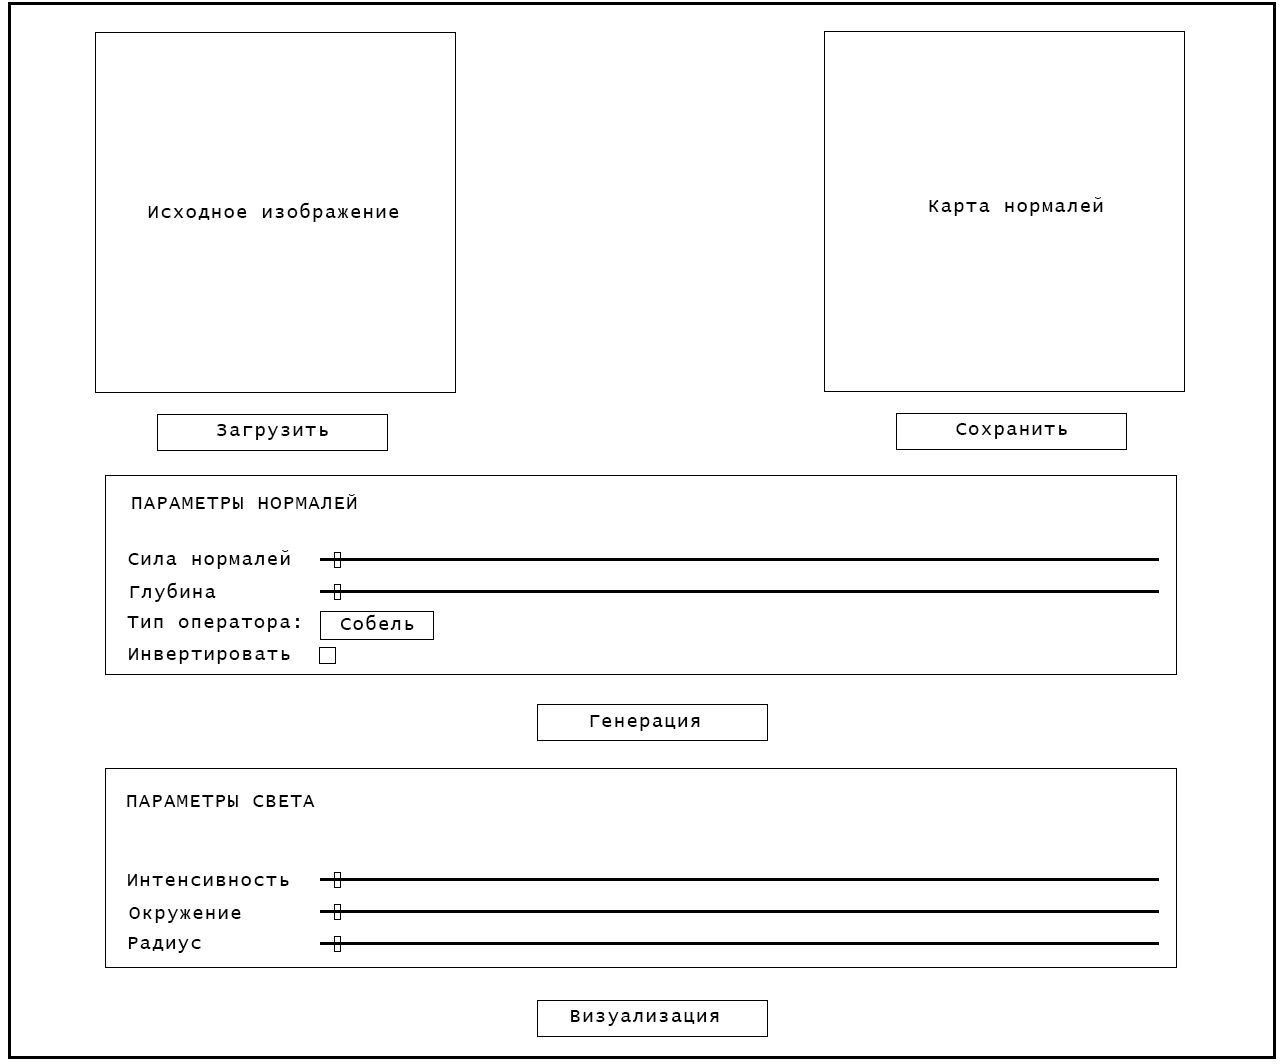
\includegraphics[width=1\linewidth]{mak}
	\caption{Макет приложения}
	\label{mak:image}
\end{figure}
\paragraph{Программные требования}

Для реализации программной информационной системы генерации карт нормалей из 2D-изображений и их визуализации используется язык программирования Python версии не ниже 3.10. Данный язык был выбран ввиду его гибкости, широкого набора библиотек для обработки изображений и создания графических интерфейсов, а также активного сообщества [19].

При разработке используются следующие библиотеки и инструменты:
\begin{enumerate}
	\item PyQt5 — для построения графического интерфейса пользователя.
	\item OpenCV — для обработки изображений, включая применение операторов градиента (Sobel, Scharr, Prewitt).
	\item NumPy — для численных операций и работы с массивами данных.
	\item Pillow (PIL) — для загрузки и сохранения изображений.
\end{enumerate}

Программа является десктопным приложением и предназначена для запуска на операционных системах Windows 10/11.

Минимальные версии компонентов:
\begin{itemize}
	\item Python 3.10+;
	\item OpenCV 4.5+;
	\item PyQt5 5.15+;
	\item NumPy 1.21+.
\end{itemize}
\paragraph{Аппаратные требования}

Для корректной работы программной системы требуется следующее минимальное аппаратное обеспечение:
\begin{enumerate}
	\item Центральный процессор: 4-ядерный с частотой не ниже 2.0 ГГц (рекомендуется ≥ 6 ядер).
	\item Оперативная память: минимум 8 ГБ (рекомендуется ≥ 16 ГБ для работы с большими изображениями).
	\item Графический процессор (опционально): для ускорения визуализации возможно использование GPU с поддержкой OpenGL 3.3 и выше.
	\item Жесткий диск: не менее 500 МБ свободного пространства для установки и хранения изображений.
	\item Разрешение экрана: минимум 1280×720 пикселей (рекомендуется 1920×1080 и выше).
	\item Операционная система: Windows 10/11.
\end{enumerate}

Наличие подключения к интернету не является обязательным для работы программы, но может использоваться при обновлениях или загрузке дополнительных изображений с онлайн-источников.
\paragraph{Требования к надёжности}

Разрабатываемое приложение представляет собой десктопную программу, работающую в автономном режиме без необходимости постоянного подключения к сети Интернет. Однако, несмотря на это, могут возникать ситуации, при которых необходима высокая устойчивость и корректное поведение приложения.

Возможные непредвиденные ситуации при работе программы:
\begin{enumerate}
	\item Преждевременное завершение работы из-за аварийного завершения ОС (например, выключение ПК, перезагрузка).
	\item Некорректное изображение или файл, не соответствующий ожидаемому формату.
	\item Отсутствие доступа к диску (например, при попытке сохранить файл на недоступный путь).
	\item Ошибки при работе с внешними библиотеками или повреждёнными изображениями.
\end{enumerate}

Меры повышения надёжности:
\begin{enumerate}
	\item Обработка всех исключений, связанных с загрузкой, сохранением и визуализацией изображений.
	\item Проверка корректности форматов данных до начала обработки.
	\item Автоматическое уведомление пользователя об ошибке с понятным описанием причины.
\end{enumerate}
\paragraph{Требования к оформлению документации}

Требования к стадиям разработки программ и программной документации для вычислительных машин, комплексов и систем независимо от их назначения и области применения, этапам и содержанию работ устанавливаются ГОСТ 19.102–77.

Программная документация должна включать в себя:
\begin{enumerate}
	\item Анализ предметной области.
	\item Техническое задание.
	\item Технический проект.
	\item Рабочий проект.	
\end{enumerate}
\subsection{Входные и выходные данные}

Данный раздел описывает, с какими данными работает разрабатываемая программно-информационная система на входе и выходе. Это необходимо для понимания характера обрабатываемой информации, форматов файлов и способов интерпретации результатов пользователем [20].
\subsubsection{Входные данные}

Входными данными для программного продукта являются:
\begin{enumerate}
	\item 2D-изображение (текстура). Пользователь может загрузить произвольное изображение, которое будет использоваться для генерации карты нормалей. Поддерживаются следующие форматы:
	\begin{itemize}
		\item PNG (.png);
		\item JPEG (.jpg, .jpeg).
	\end{itemize}
	\item Параметры генерации нормалей, устанавливаемые через пользовательский интерфейс:
	\begin{itemize}
		\item оператор градиента: выбор между Sobel, Scharr, Prewitt;
		\item сила нормалей (амплитуда влияния градиента);
		\item глубина нормалей (масштаб Z-компоненты);
		\item инверсия нормалей (по оси X, Y, Z);
		\item размер ядра фильтра (при наличии настройки);
		\item цветовое пространство: при необходимости — выбор канала обработки (например, яркость, средний цвет, градации серого).
	\end{itemize}	
	\item Параметры визуализации:
	\begin{itemize}
		\item интенсивность света (яркость источника);
		\item радиус фонарика (область действия);
		\item положение источника света (движение мышью в интерактивном режиме).
	\end{itemize}	
\end{enumerate}

Все параметры могут быть изменены пользователем до или после загрузки изображения. Программа немедленно пересчитывает результат при изменении параметров.
\subsubsection{Выходные данные}

Выходные данные делятся на основные (результаты генерации) и вспомогательные (визуализация, сохранение):
\begin{enumerate}
	\item Карта нормалей представлена в виде цветного изображения, где:
	\begin{itemize}
		\item формат файла: PNG (бессжатый);
		\item цветовое пространство — стандартное RGB;
	\end{itemize}	
	\item Визуализированная текстура с освещением:
	\begin{itemize}
		\item представляет собой наложение карты нормалей на исходную текстуру с учётом виртуального освещения;
		\item реализация через симуляцию источника света, перемещаемого мышью;
		\item выходной формат: PNG.
	\end{itemize}	
\end{enumerate}
\subsection{Варианты использования}

Диаграмма прецендентов представлена на рисунке ~\ref{prec:image}.

\begin{figure}[ht]
	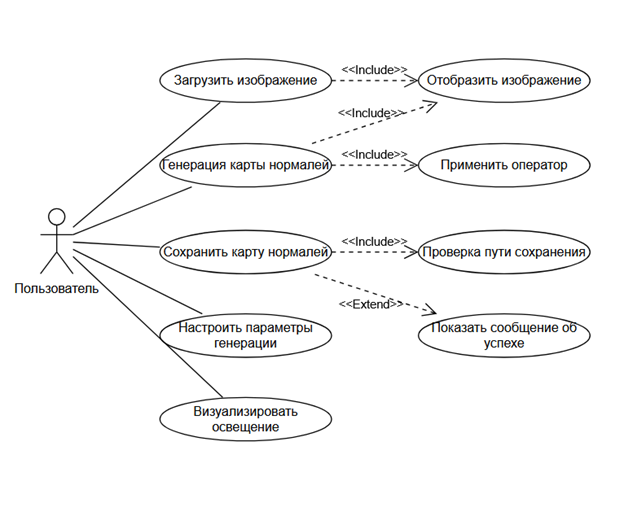
\includegraphics[width=1\linewidth]{prec}
	\caption{Диаграмма прецендентов}
	\label{prec:image}
\end{figure}
\subsubsection{Вариант использования «Загрузка изображения»}

Заинтересованные лица и их требования: пользователь хочет загрузить своё изображение (например, текстуру) в приложение, чтобы сгенерировать карту нормалей.

Предусловие: приложение запущено. Пользователь находится на вкладке генерации.

Постусловие: изображение отображается в левой части интерфейса, готовое к дальнейшей обработке.

Основной успешный сценарий:
\begin{enumerate}
	\item Пользователь нажимает кнопку «Загрузить».
	\item Система открывает диалог выбора файла.
	\item Пользователь выбирает изображение в поддерживаемом формате (PNG, JPG и др.).
	\item Система загружает изображение и отображает его на панели.
	\item Пользователь может перейти к следующему действию — генерации карты нормалей.
\end{enumerate}
\subsubsection{Вариант использования «Генерация карты нормалей»}

Заинтересованные лица и их требования: пользователь хочет создать карту нормалей из загруженного изображения.

Предусловие: загружено изображение, выбран алгоритм генерации и параметры (например, оператор Собеля, глубина).

Постусловие: система сгенерировала карту нормалей и отобразила её в правой части интерфейса.

Основной успешный сценарий:
\begin{enumerate}
	\item Пользователь настраивает параметры генерации (оператор, инверсия, глубина и т.д.).
	\item Пользователь нажимает кнопку «Сгенерировать».
	\item Система применяет выбранный алгоритм к изображению.
	\item Результат отображается в виде карты нормалей.
\end{enumerate}
\subsubsection{Вариант использования «Сохранение карты нормалей»}

Заинтересованные лица и их требования: пользователь хочет сохранить сгенерированную карту нормалей для дальнейшего использования.

Предусловие: карта нормалей сгенерирована и отображена в правой панели.

Постусловие: изображение с картой нормалей сохранено в выбранную папку.

Основной успешный сценарий:
\begin{enumerate}
	\item Пользователь нажимает кнопку «Сохранить».
	\item Открывается диалог выбора пути сохранения.
	\item Пользователь указывает имя файла и формат (PNG).
	\item Система сохраняет изображение.
\end{enumerate}
\subsubsection{Вариант использования «Интерактивная визуализация»}

Заинтересованные лица и их требования: пользователь хочет увидеть, как карта нормалей влияет на освещение изображения при движении источника света.

Предусловие: карта нормалей сгенерирована.

Постусловие: пользователь может видеть результат освещения в реальном времени, двигая мышь как источник света.

Основной успешный сценарий:
\begin{enumerate}
	\item Пользователь нажимает кнопку «Визуализировать».
	\item Система активирует режим визуализации с освещением.
	\item Пользователь перемещает курсор мыши, который действует как источник света.
	\item Система обновляет освещённость изображения в зависимости от карты нормалей и положения света.
\end{enumerate}
\subsubsection{Вариант использования «Настройка параметров освещения»}

Заинтересованные лица и их требования: пользователь хочет изменить параметры освещения, такие как интенсивность и радиус, чтобы лучше видеть рельеф по нормалям.

Предусловие: активирован режим визуализации.

Постусловие: сцена обновляется в соответствии с новыми параметрами.

Основной успешный сценарий:
\begin{enumerate}
	\item Пользователь регулирует ползунки интенсивности и радиуса света.
	\item Система обновляет визуализацию освещения.
\end{enumerate}
\subsubsection{Вариант использования «Выбор оператора генерации»}

Заинтересованные лица и их требования: пользователь хочет протестировать разные алгоритмы (например, Собель, Шарра, Превитт) для генерации карты нормалей и выбрать оптимальный.

Предусловие: загружено исходное изображение.

Постусловие: выбранный алгоритм применяется при генерации карты нормалей.

Основной успешный сценарий:
\begin{enumerate}
	\item Пользователь открывает выпадающий список с доступными операторами.
	\item Пользователь выбирает нужный оператор.
	\item Выбор сохраняется в параметрах генерации.
	\item При нажатии «Сгенерировать» применяется выбранный оператор.
\end{enumerate}
\subsubsection{Вариант использования «Инвертирование нормалей»}

Заинтересованные лица и их требования: пользователь хочет инвертировать карту нормалей, чтобы изменить визуальное восприятие рельефа.

Предусловие: выставлены параметры генерации, изображение загружено.

Постусловие: генерируется инвертированная карта нормалей.

Основной успешный сценарий:
\begin{enumerate}
	\item Пользователь активирует чекбокс «Инвертировать нормали».
	\item Нажимает «Сгенерировать».
	\item Система создаёт инвертированную карту.
	\item Результат отображается в интерфейсе.
\end{enumerate}
\subsubsection{Вариант использования «Настройка глубины нормалей»}

Заинтересованные лица и их требования: пользователь хочет усилить или ослабить эффект рельефа при визуализации.

Предусловие: загружено изображение, активен режим генерации.

Постусловие: карта нормалей учитывает заданный уровень глубины при расчёте векторов.

Основной успешный сценарий:
\begin{enumerate}
	\item Пользователь перемещает ползунок глубины нормалей.
	\item Значение используется при генерации.
	\item Пользователь нажимает «Сгенерировать».
	\item Карта нормалей обновляется с учётом новой глубины.
\end{enumerate}
\section{Технический проект}
\subsection{Общая характеристика организации решения задачи}

Разрабатываемая система представляет собой настольное приложение, позволяющее пользователю выполнять две ключевые задачи: построение карт нормалей по двумерным изображениям и интерактивную визуализацию полученных данных с имитацией освещения \cite{tidwell2020}.

Архитектура приложения построена по модульному принципу, что обеспечивает независимость компонентов, удобство расширения и тестирования, а также простоту поддержки. Вся логика работы разделена на два ключевых функциональных блока:

\begin{enumerate}
	\item Модуль генерации карт нормалей. Этот компонент отвечает за обработку загруженного 2D-изображения и построение карты нормалей с помощью градиентного анализа. Пользователь может выбрать один из трёх алгоритмов: Sobel, Scharr или Prewitt. Каждый из них позволяет выявлять локальные изменения яркости изображения и формировать на их основе вектор нормали. В дополнение к алгоритму доступны параметры настройки: сила нормалей, глубина, инверсия. Все изменения применяются в реальном времени, что позволяет интерактивно наблюдать результат и адаптировать карту под нужды конкретной текстуры. Полученная карта нормалей автоматически сохраняется в памяти и используется далее при визуализации.
	\item Модуль визуализации предоставляет пользователю два режима анализа результатов: 2D-визуализацию и 3D-визуализацию.
	\begin{enumerate}[label=\theenumi.\arabic*.]
		\item В 2D-режиме используется техника имитации направленного света («фонарика»), управляемого движением курсора мыши. На основе нормалей рассчитывается освещённость каждой точки изображения, учитывая интенсивность и радиус света, а также уровень фоновой засветки. Таким образом создаётся реалистичный эффект освещения, позволяющий оценить, как текстура будет выглядеть в игровых сценах.
		\item В 3D-режиме карта нормалей и текстура проецируются на все шесть граней виртуального куба, который визуализируется с использованием OpenGL посредством GLCubeWidget. Пользователь может вращать куб мышью, изменяя ракурс наблюдения, и наблюдать взаимодействие нормалей с направленным освещением. Параметры света остаются настраиваемыми -- интенсивность, радиус действия и рассеянность. Это расширяет возможности анализа и делает приложение более гибким в применении к задачам геймдизайна и графического моделирования.
	\end{enumerate}
\end{enumerate}

Поддержка как 2D-, так и 3D-визуализации позволяет пользователю выбирать наиболее подходящий способ анализа текстуры в зависимости от задачи: от быстрой проверки нормалей в плоскости -- до полноценного пространственного анализа поведения света. Такое архитектурное разделение обеспечивает гибкость, модульность и расширяемость приложения.

Графический интерфейс реализован с использованием библиотеки PyQt5 и спроектирован с учётом требований к удобству пользователя \cite{prokhorenok2021}. Все элементы интерфейса размещены логично: процесс работы разбит на этапы (загрузка изображения, генерация нормалей, визуализация), элементы управления параметрами имеют понятные подписи и расположение, соответствующее разработанному макету \cite{cooper2020}.
\subsection{Обоснование выбора технологий проектирования}

При разработке программно-информационной системы создания карт нормалей и их визуализации был проведён анализ различных языков программирования и программных библиотек, применимых для решения задач в области компьютерной графики, обработки изображений и создания пользовательского интерфейса. В результате был выбран стек технологий, оптимально сочетающий простоту разработки, функциональные возможности и широкую поддержку со стороны сообщества.
\subsubsection{Язык программирования: Python}

Python был выбран как основной язык разработки благодаря своей читаемости, лаконичному синтаксису и возможности быстрой реализации алгоритмов, что особенно важно при построении интерактивных приложений. Он активно используется в научных и прикладных областях, включая обработку изображений, машинное обучение и визуализацию данных. Кроме того, кроссплатформенность Python позволяет запускать приложение на различных операционных системах, а большое сообщество и развитая экосистема делают процесс разработки и отладки значительно проще \cite{ravichandiran2020}.
\subsubsection{PyQt5}

PyQt5 -- библиотека для создания графического интерфейса. Для реализации графического интерфейса была выбрана библиотека PyQt5 -- привязка Python к мощному C++ фреймворку Qt \cite{talipov2020}. Основные причины выбора:
\begin{enumerate}
	\item Поддержка широкого спектра элементов интерфейса: кнопки, панели, слайдеры, вкладки и другие виджеты.
	\item Гибкая настройка расположения элементов -- реализована возможность построения интерфейсов, соответствующих пользовательским макетам.
	\item Событийно-ориентированная модель -- облегчает обработку пользовательских взаимодействий (например, загрузка изображений, перемещение мыши).
	\item Интеграция с другими библиотеками Python -- PyQt5 хорошо работает в связке с NumPy, OpenCV и другими модулями.
\end{enumerate}
\subsubsection{OpenCV и NumPy}

OpenCV и NumPy -- библиотеки для обработки изображений. Для обработки изображений и реализации операторов градиентного анализа были использованы библиотеки:
\begin{enumerate}
	\item OpenCV -- открытая библиотека для обработки изображений и компьютерного зрения \cite{kaehler2021}. Обеспечивает эффективную реализацию операторов Sobel, Scharr и Prewitt, а также позволяет выполнять фильтрацию, преобразования, нормализацию и другие операции.
	\item NumPy -- библиотека для работы с многомерными массивами и матрицами. Активно используется для хранения изображений в числовом формате, выполнения математических операций над данными пикселей и ускорения вычислений.
\end{enumerate}
\subsubsection{Pillow}

Pillow -- библиотека для загрузки и сохранения изображений. Для работы с форматами изображений (PNG, JPG и др.) используется библиотека Pillow, являющаяся модернизированной и расширенной версией PIL (Python Imaging Library). Она позволяет:
\begin{enumerate}
	\item Загружать изображения из файлов.
	\item Конвертировать изображения между различными цветовыми пространствами.
	\item Сохранять результаты генерации нормалей в различных форматах.
	\item Извлекать метаинформацию об изображениях.
\end{enumerate}

\subsubsection{OpenGL}
OpenGL -- библиотека для трёхмерной графики и визуализации.
С использованием OpenGL реализованы следующие возможности:
\begin{enumerate}
	\item Создание 3D-сцены с кубом, каждая грань которого текстурирована загруженным изображением.
	\item Назначение карты нормалей в качестве источника данных для расчёта взаимодействия поверхности с направленным освещением.
	\item Обработка пользовательского ввода (вращение, масштабирование сцены).
	\item Моделирование поведения направленного источника света и реалистичного освещения с учётом нормалей.
\end{enumerate}
\begin{comment}
Python был выбран в качестве основного языка разработки по следующим причинам:
\begin{enumerate}
	\item Простота синтаксиса и высокая читаемость кода — это позволяет быстро реализовывать алгоритмы, минимизируя вероятность ошибок и снижая порог входа для других разработчиков \cite{ravichandiran2020}.
	\item Большое количество библиотек для работы с изображениями и интерфейсом — Python активно используется в научной и прикладной разработке в области компьютерного зрения.
	\item Кроссплатформенность — Python-приложения можно запускать под различными операционными системами, включая Windows, Linux и macOS.
	\item Активное сообщество и широкая документация — в случае возникновения проблем легко найти решение или получить помощь.
\end{enumerate}
\subsubsection{PyQt5}

PyQt5 — библиотека для создания графического интерфейса. Для реализации графического интерфейса была выбрана библиотека PyQt5 — привязка Python к мощному C++ фреймворку Qt \cite{talipov2020}. Основные причины выбора:
\begin{enumerate}
	\item Поддержка широкого спектра элементов интерфейса: кнопки, панели, слайдеры, вкладки и другие виджеты.
	\item Гибкая настройка расположения элементов — реализована возможность построения интерфейсов, соответствующих пользовательским макетам.
	\item Событийно-ориентированная модель — облегчает обработку пользовательских взаимодействий (например, загрузка изображений, перемещение мыши).
	\item Интеграция с другими библиотеками Python — PyQt5 хорошо работает в связке с NumPy, OpenCV и другими модулями.
\end{enumerate}
\subsubsection{OpenCV и NumPy}

OpenCV и NumPy — библиотеки для обработки изображений. Для обработки изображений и реализации операторов градиентного анализа были использованы библиотеки:
\begin{enumerate}
	\item OpenCV — открытая библиотека для обработки изображений и компьютерного зрения \cite{kaehler2021}. Обеспечивает эффективную реализацию операторов Sobel, Scharr и Prewitt, а также позволяет выполнять фильтрацию, преобразования, нормализацию и другие операции.
	\item NumPy — библиотека для работы с многомерными массивами и матрицами. Активно используется для хранения изображений в числовом формате, выполнения математических операций над данными пикселей и ускорения вычислений.
\end{enumerate}
\subsubsection{Pillow}

Pillow — библиотека для загрузки и сохранения изображений. Для работы с форматами изображений (PNG, JPG и др.) используется библиотека Pillow, являющаяся модернизированной и расширенной версией PIL (Python Imaging Library). Она позволяет:
\begin{enumerate}
	\item Загружать изображения из файлов.
	\item Конвертировать изображения между различными цветовыми пространствами.
	\item Сохранять результаты генерации нормалей в различных форматах.
	\item Извлекать метаинформацию об изображениях.
\end{enumerate}

OpenGL — библиотека для трёхмерной графики и визуализации.
С использованием OpenGL реализованы следующие возможности:
\begin{enumerate}
	\item Создание 3D-сцены с кубом, каждая грань которого текстурирована загруженным изображением.
	\item Назначение карты нормалей в качестве источника данных для расчёта взаимодействия поверхности с направленным освещением.
	\item Обработка пользовательского ввода (вращение, масштабирование сцены).
	\item Моделирование поведения направленного источника света и реалистичного освещения с учётом нормалей.
\end{enumerate}

Для отображения визуального эффекта освещения по нормалям применяется рендеринг на холст с использованием комбинации данных карты нормалей и положения мыши. Алгоритм реализован вручную с использованием NumPy и PyQt5, без сторонних движков визуализации, что обеспечивает наглядность и полный контроль над процессом.
\end{comment}
\subsection{Общая архитектура системы}

Программно-информационная система генерации карт нормалей и их интерактивной визуализации построена по модульному принципу. Это обеспечивает высокую модульность, возможность масштабирования и упрощает сопровождение и тестирование. Приложение реализовано как настольное, с графическим интерфейсом на языке Python. Система поддерживает два режима визуализации: в 2D с имитацией освещения и в 3D с использованием OpenGL.

Диаграмма компонентов представлена на рисунке~\ref{comp2:image}.

\begin{figure}[ht]
	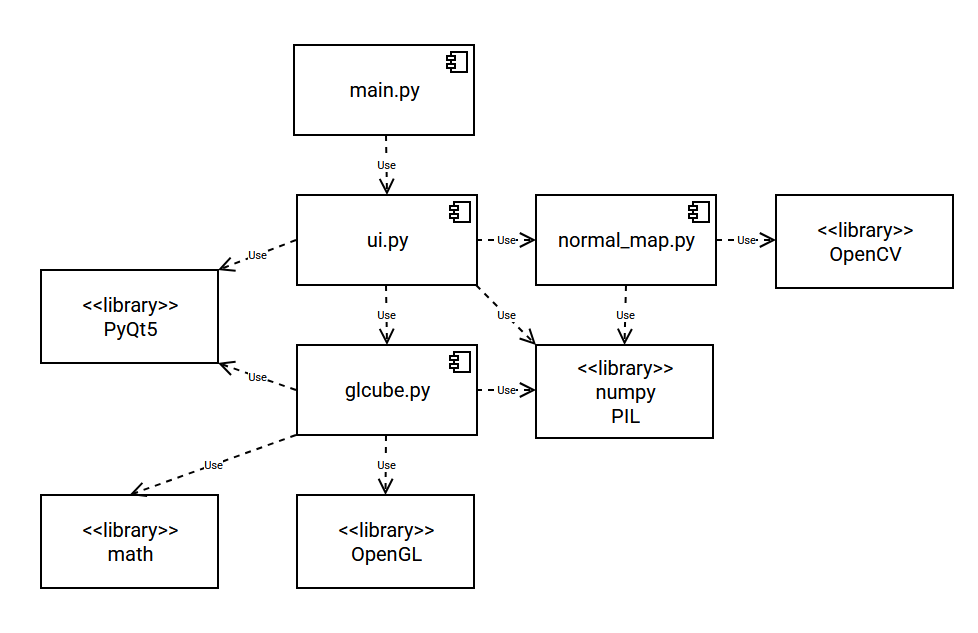
\includegraphics[width=1\linewidth]{comp2}
	\caption{Диаграмма компонентов программной системы}
	\label{comp2:image}
\end{figure}

Основные модули системы:

\begin{enumerate}
	\item Интерфейсный и логический модуль -- файл ui.py.
	\item Модуль генерации карты нормалей -- файл normal\_map.py.
	\item Модуль визуализации в 3D -- файл glcube.py.
	\item Точка входа в приложение -- файл main.py.
\end{enumerate}

\subsubsection{Интерфейсный и логический модуль (ui.py)}

Этот модуль содержит основную логику работы программы и формирует графический интерфейс при помощи библиотеки PyQt5. Все взаимодействия с пользователем происходят именно в этом модуле: действия передаются в модуль генерации нормалей или в OpenGL-виджет. В ui.py реализованы:

\begin{enumerate}
	\item Загрузка изображения (PNG, JPEG, BMP) через диалог выбора файла.
	\item Управление параметрами генерации карты нормалей: выбор оператора (Sobel, Scharr, Prewitt), сила, глубина, инверсия.
	\item Отображение оригинального изображения и сгенерированной карты нормалей.
	\item Визуализация эффекта освещения в 2D режиме -- поведение источника света («фонарика») следует за движением курсора.
	\item Отображение изображения с освещением в реальном времени.
	\item Переключение между 2D и 3D режимами.
	\item Сохранение сгенерированной карты нормалей.
\end{enumerate}

\subsubsection{Модуль генерации нормалей (normal\_map.py)}

Функциональность, связанная с построением карты нормалей на основе изображения, реализована в модуле normal\_map.py. Он предоставляет реализацию нескольких алгоритмов обработки: оператор Собеля, позволяющий вычислять производные первого порядка, оператор Шарра -- более чувствительный к границам, а также оператор Превитта -- простой, но быстрый метод вычисления градиентов. Эти методы позволяют проанализировать локальные изменения яркости изображения и, на их основе, сформировать векторные направления.

Модуль принимает на вход изображение, масштабирует и анализирует его, а затем создаёт нормаль-карту -- изображение, в котором каждый пиксель содержит направление нормали, закодированное в цветовых каналах RGB. Пользователь может регулировать параметры: сила нормалей определяет масштаб по осям X и Y, глубина влияет на составляющую по оси Z, а параметр инверсии меняет направление нормалей на противоположное. Этот модуль полностью автономен и предоставляет интерфейс для подключения к визуализаторам.
\subsubsection{Модуль визуализации в 3D (glcube.py)}

Трёхмерный режим работы реализован в модуле glcube.py, где используется QOpenGLWidget в связке с библиотекой PyOpenGL. Этот компонент отвечает за отрисовку куба, на грани которого накладываются текстура и карта нормалей. Задача -- предоставить пользователю возможность оценить, как освещение взаимодействует с нормалями в пространстве. Модуль осуществляет преобразование изображений в формат, пригодный для загрузки в виде OpenGL-текстур, после чего каждая грань куба получает свой визуальный слой.

Пользователь может вращать куб мышью, изменять масштаб изображения, управлять положением виртуального источника света. Благодаря встроенным функциям расчёта взаимодействия света с нормалями создаётся реалистичная симуляция поведения материала под разными углами обзора и освещённости. Это расширяет возможности анализа и делает приложение полезным в задачах трёхмерного дизайна и текстурирования.

\subsubsection{Точка входа (main.py)}

Файл main.py играет вспомогательную роль. Он содержит лишь минимальный код, необходимый для запуска программы. Основной задачей данного файла является импорт основного класса интерфейса из ui.py, инициализация приложения и передача управления в главный цикл событий. Таким образом, этот модуль является точкой входа в систему и отвечает за запуск всей программной инфраструктуры.
\subsection{Реализация модуля генерации карт нормалей}

Модуль генерации нормалей выполняет задачу преобразования двухмерного изображения в нормал-карту -- изображение с закодированной информацией о направлении нормалей к условной поверхности. Это позволяет воссоздавать визуальное ощущение рельефа без увеличения геометрической сложности сцены \cite{russ2020}.

Алгоритм построения нормалей реализован в несколько этапов, последовательно обрабатывающих входное изображение.

На первом шаге происходит преобразование изображения в полутоновый формат. Перевод в оттенки серого необходим для устранения цветовой информации, которая не влияет на вычисление нормалей, и упрощает последующие операции. Далее изображение представляется в виде числового массива яркостных значений, пригодного для вычислений.

Следующий этап включает расчёт градиентов яркости по горизонтальной и вертикальной осям. Для этого применяется один из стандартных операторов свёртки -- Sobel, Scharr или Prewitt. Выбор осуществляется пользователем через интерфейс приложения. Эти операторы определяют направление и интенсивность изменения яркости, что позволяет судить о локальной «высоте» каждого участка изображения.

Вычисленные значения градиента масштабируются по заданному пользователем параметру силы нормалей. Этот параметр влияет на степень выраженности рельефа: чем выше значение, тем сильнее акцентируются перепады высоты. Компонента нормали вдоль оси Z (глубины) берётся как константа, модифицируемая параметром глубины.

На основе всех трёх компонент (X, Y, Z) формируется вектор нормали. Все векторы проходят процедуру нормализации, приводящую их к единичной длине. Это необходимо для корректной интерпретации направлений в графической визуализации.

Дополнительно реализована опция инверсии: при её включении направления нормалей зеркально отражаются. Такая возможность обеспечивает совместимость с различными движками, где ориентация нормалей может интерпретироваться по-разному.

На завершающем этапе нормализованные векторы преобразуются в изображение: их значения сжимаются в диапазон [0; 1] и распределяются по цветовым каналам RGB. Полученная нормал-карта возвращается в виде изображения, пригодного для последующей визуализации в 2D и 3D, а также может быть сохранена пользователем в файл \cite{day2021}.

Таким образом, модуль реализует надёжный и расширяемый алгоритм генерации нормалей, позволяющий создавать качественные псевдорельефные карты из любых 2D-текстур. Гибкие параметры и поддержка нескольких операторов позволяют адаптировать результат под конкретные задачи в визуализации и игровых проектах.
\subsection{Реализация модуля визуализации освещения}

Модуль визуализации освещения предназначен для отображения результатов генерации карты нормалей с учётом воздействия направленного источника света. В системе реализованы два режима визуализации: 2D-режим, где эффект освещения имитируется на плоской текстуре, и 3D-режим, в котором карта нормалей применяется на грани трёхмерного куба.
\subsubsection{2D-визуализация}

После загрузки изображения и генерации карты нормалей система автоматически визуализирует результат на основе положения курсора мыши, выполняющего роль направленного источника света. Освещённость пересчитывается в реальном времени при каждом движении мыши.

Алгоритм работы следующий:
\begin{enumerate}
	\item Пользователь перемещает курсор над областью изображения.
	\item Программа фиксирует координаты мыши как положение источника света.
	\item Для каждой точки изображения рассчитывается вектор от пикселя к источнику света.
	\item Система нормализует вектор направления света и нормаль из карты.
	\item Вычисляется скалярное произведение между нормалью и вектором света.
	\item Полученное значение модифицируется с учётом: радиуса действия света, фоновой освещённости, интенсивности света.
	\item Яркость каждого пикселя обновляется в соответствии с результатами расчёта.
	\item Обновлённое изображение отображается в интерфейсе.
\end{enumerate}
\subsubsection{3D-визуализация}

В 3D-режиме карта нормалей применяется к поверхности куба, визуализируемого при помощи OpenGL. Каждая грань отображает исходное изображение с имитацией объёмности за счёт световых эффектов.

Алгоритм работы 3D-режима:
\begin{enumerate}
	\item После переключения в режим 3D запускается компонент QOpenGLWidget.
	\item Выполняется инициализация сцены и загрузка текстур.
	\item Куб отображается на экране с наложением изображения и нормалей.
	\item Пользователь может вращать куб мышью, меняя угол обзора.
	\item Источник света фиксирован в сцене и направлен в центр объекта.
	\item Для каждой вершины и фрагмента куба применяется освещение на основе нормалей.
	\item Освещение рассчитывается с использованием OpenGL, включая нормализацию, модель Ламберта и затухание.
	\item Сцена обновляется в реальном времени.
\end{enumerate}
\subsection{Структура пользовательского интерфейса}

На основании требований к пользовательскому интерфейсу, представленных в пункте 2.3.2.1 технического задания, был разработан графический интерфейс приложения. Интерфейс реализован с использованием библиотеки PyQt5, которая позволяет создать графическое приложение с гибкой системой компоновки элементов и поддержкой событий.

Интерфейс программы представлен на рисунке ~\ref{interf2:image}.

\begin{figure}[ht]
	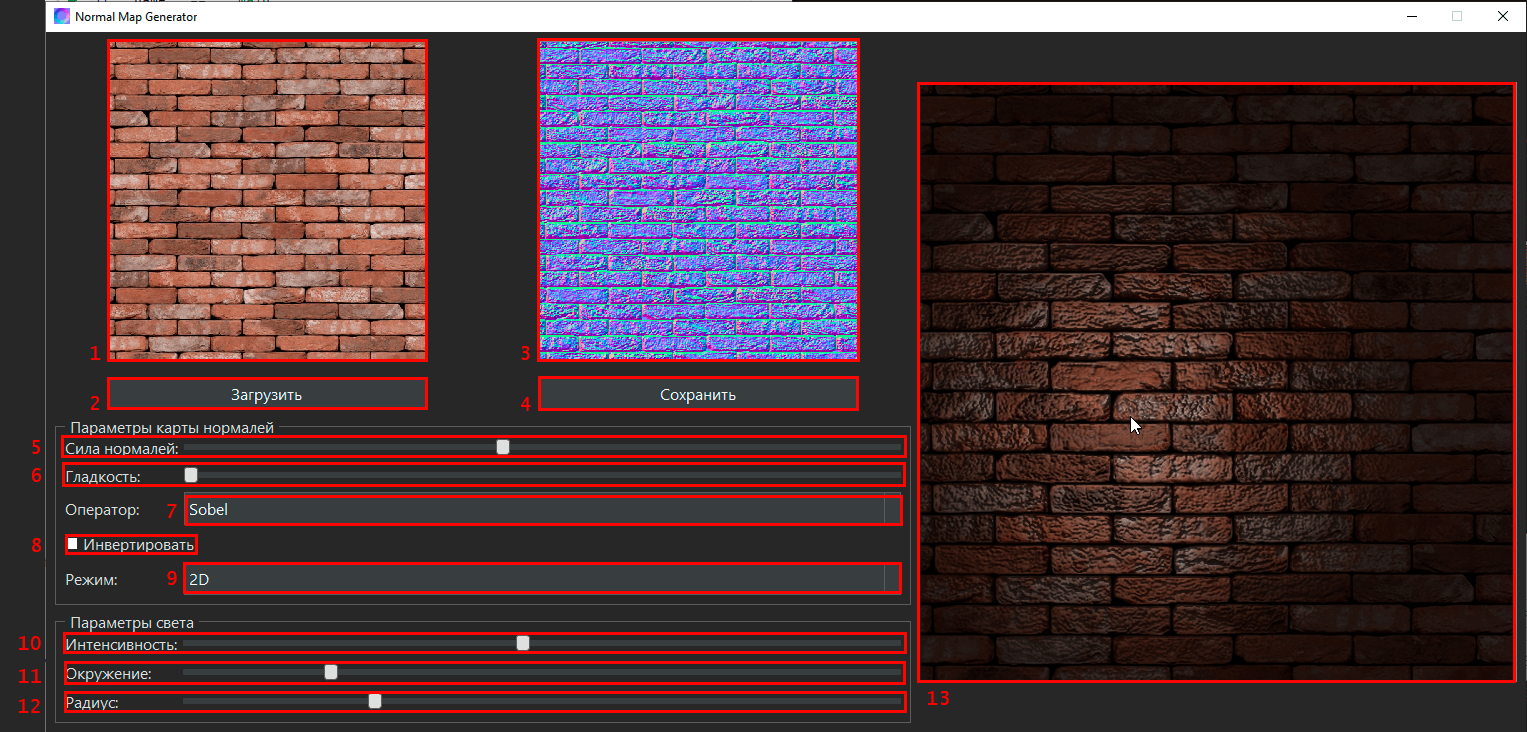
\includegraphics[width=1\linewidth]{interf2}
	\caption{Интерфейс программы}
	\label{interf2:image}
\end{figure}

Элементы интерфейса:
\begin{enumerate}
	\item Окно оригинального изображения. Отображает исходное изображение, загруженное пользователем для генерации карты нормалей.
	\item Кнопка «Загрузить». Открывает диалоговое окно выбора изображения, которое будет использоваться для анализа и генерации нормалей.	
	\item Окно карты нормалей. Показывает сгенерированную карту нормалей на основе оригинального изображения и выбранных параметров.
	\item Кнопка «Сохранить». Сохраняет сгенерированную карту нормалей в выбранное пользователем место.
	\item Ползунок «Сила нормалей». Регулирует интенсивность/амплитуду нормалей. Чем выше значение, тем рельефнее выглядит результат.
	\item Ползунок «Гладкость». Активирует дополнительное влияние глубины на расчет нормалей (если предусмотрена соответствующая логика в коде).
	\item Выпадающий список «Оператор». Позволяет выбрать математический оператор, применяемый для выделения границ (например, Собель, Шарра и др.).
	\item Чекбокс «Инвертировать». При включении инвертирует направление нормалей, меняя визуальное восприятие рельефа.
	\item Выпадающий список «Режим». Позволяет выбрать режим отображения визуализации (2D и 3D).	
	\item Ползунок «Интенсивность». Управляет яркостью источника света при визуализации эффекта освещения.
	\item Ползунок «Окружение». Добавляет равномерное базовое освещение всей сцены для повышения читаемости изображения.
	\item  Ползунок «Радиус». Определяет зону, охватываемую виртуальным «фонариком». Чем больше значение, тем шире область освещённости.
	\item Окно визуализации. Показывает изображение с наложенной картой нормалей, в котором курсор мыши используется как источник света для динамического освещения по карте нормалей.
\end{enumerate}

\ifПрактика{}\else{
   \section{Рабочий проект}
\subsection{Классы, используемые при разработке}

В процессе разработки программной информационной системы были использованы различные классы, каждый из которых выполняет строго определённую функцию в архитектуре приложения. В таблице \ref{class:table} приведён перечень ключевых классов, описание их назначения, модули, в которых они реализованы, а также перечень основных методов. Такая структура помогает обеспечить модульность, читаемость и масштабируемость системы.

\renewcommand{\arraystretch}{0.8} % уменьшение расстояний до сетки таблицы
\begin{xltabular}{\textwidth}{|X|p{2.5cm}|>{\setlength{\baselineskip}{0.7\baselineskip}}p{4.85cm}|>{\setlength{\baselineskip}{0.7\baselineskip}}p{4.85cm}|}
	\caption{Описание классов, используемых в приложении\label{class:table}}\\
	\hline \centrow \setlength{\baselineskip}{0.7\baselineskip} Название класса & \centrow \setlength{\baselineskip}{0.7\baselineskip} Модуль, к которому относится класс & \centrow Описание класса & \centrow Методы \\
	\hline \centrow 1 & \centrow 2 & \centrow 3 & \centrow 4\\ \hline
	\endfirsthead
	\caption*{Продолжение таблицы \ref{class:table}}\\
	\hline \centrow 1 & \centrow 2 & \centrow 3 & \centrow 4\\ \hline
	\finishhead
	NormalMap\allowbreak App & main.py & Главный класс графического интерфейса. Управляет загрузкой изображения, генерацией нормалей, запуском визуализации и отображением результата. & load\_image(), generate\_normal\_map(), visualize(), save\_output()\\
	\hline GLCube\allowbreak Widget & glcube.py & OpenGL -- виджет для визуализации карты нормалей в 3D-режиме. Отвечает за отображение куба и освещения. & initializeGL(), paintGL(), resizeGL()
\end{xltabular}
\renewcommand{\arraystretch}{1.0} % восстановление сетки

\subsection{Функции программной системы}

Программная система состоит из набора функций, каждая из которых отвечает за конкретную задачу в рамках обработки изображений, генерации карт нормалей или визуализации результата. Таблица \ref{func:table} содержит список основных функций, описание их назначения и указание на модули, где они применяются.

\renewcommand{\arraystretch}{0.8} % уменьшение расстояний до сетки таблицы
\begin{xltabular}{\textwidth}{|p{4.85cm}|>{\setlength{\baselineskip}{0.7\baselineskip}}p{2.5cm}|X|>{\setlength{\baselineskip}{0.7\baselineskip}}p{4.85cm}|}
	\caption{Описание функций, используемых в приложении\label{func:table}}\\
	\hline \centrow \setlength{\baselineskip}{0.7\baselineskip} Название функции & \centrow \setlength{\baselineskip}{0.7\baselineskip} Модуль, к которому относится функция & \centrow Назначение \\
	\hline \centrow 1 & \centrow 2 & \centrow 3\\ \hline
	\endfirsthead
	\caption*{Продолжение таблицы \ref{func:table}}\\
	\hline \centrow 1 & \centrow 2 & \centrow 3\\ \hline
	\finishhead
	\_\_init\_\_(self) & ui.py & Конструктор главного окна. Инициализирует интерфейс и параметры.\\
	\hline update\_strength(self, value) & ui.py & Обновляет значение силы градиента по слайдеру. \\
	\hline update\_depth(self, value) & ui.py & Обновляет параметр глубины нормалей. \\
	\hline update\_operator(self, text) & ui.py & Устанавливает выбранный оператор градиента (Sobel, Scharr, Prewitt). \\
	\hline update\_invert(self, state) & ui.py & Включает или отключает инвертирование нормалей. \\
	\hline update\_light\_params\allowbreak(self) & ui.py & Обновляет параметры источника света (интенсивность, радиус, ambient). \\
	\hline load\_image(self) & ui.py & Загружает изображение, отображает его в интерфейсе. \\
	\hline process\_image(self) & ui.py & Генерирует карту нормалей из загруженного изображения. \\
	\hline save\_normal\_map(self) & ui.py & Сохраняет текущую карту нормалей в файл. \\
	\hline visualize(self) & ui.py & Запускает визуализацию освещения (в 2D или 3D режиме). \\
	\hline get\_shaded\_image\_for\_\allowbreak3d(self) -> Image.Image & ui.py & Создаёт изображение с освещением для использования в OpenGL. \\
	\hline update\_mode(self, text) & ui.py & Переключает режим визуализации (2D или 3D). \\
	\hline run(self) & ui.py & Запускает основное окно приложения. \\
	\hline \_\_init\_\_(self, image, parent=None) & glcube.py & Конструктор OpenGL-виджета, принимает изображение с нормалями. \\
	\hline initializeGL(self) & glcube.py & Инициализирует OpenGL-контекст и параметры отрисовки. \\
	\hline bind\_texture(self, pil\_image) & glcube.py & Привязывает текстуру к кубу из изображения. \\
	\hline resizeGL(self, w, h) & glcube.py & Обрабатывает изменение размера OpenGL-окна. \\
	\hline paintGL(self) & glcube.py & Выполняет отрисовку куба с текстурами и освещением. \\
	\hline draw\_cube(self) & glcube.py & Рисует шесть граней куба и применяет текстуры. \\
	\hline normalize(self, v) & glcube.py & Нормализует вектор, используется при расчёте освещения. \\
	\hline mousePressEvent(self, event) & glcube.py & Реагирует на нажатие мыши для вращения куба. \\
	\hline mouseMoveEvent(self, event) & glcube.py & Обрабатывает перемещение мыши для изменения ориентации куба. \\
	\hline wheelEvent(self, event) & glcube.py & Управляет масштабированием сцены с помощью колеса мыши. \\
	\hline generate\_normal\_map\allowbreak(image, strength, ...) & normal\_\allowbreak map.py & Главная функция генерации карты нормалей по изображению с параметрами. \\
	
\end{xltabular}
\renewcommand{\arraystretch}{1.0} % восстановление сетки



\subsection{Модульное тестирование разработанного web-сайта}

Модульное тестирование направлено на проверку корректной работы отдельных функциональных блоков системы \cite{ahmed2021}. Это особенно важно при разработке прикладных программ, содержащих алгоритмы обработки изображений и управляющие элементы интерфейса. Для предлагаемой информационной системы генерации карт нормалей модульное тестирование позволяет выявить ошибки в логике преобразования данных, а также убедиться в корректной работе функций по загрузке, сохранению и визуализации результатов.

Для проведения модульного тестирования использовалась встроенная библиотека unittest языка Python. Она предоставляет функциональность для написания и запуска тестов, а также фиксации результатов.

Тесты для модуля generate\_normal\_map() представлены в таблице \ref{test1:table}.

\renewcommand{\arraystretch}{0.8} % уменьшение расстояний до сетки таблицы
\begin{xltabular}{\textwidth}{|X|p{4.85cm}|>{\setlength{\baselineskip}{0.7\baselineskip}}p{3.0cm}|>{\setlength{\baselineskip}{0.7\baselineskip}}p{3.0cm}|}
	\caption{Модульные тесты для generate\_normal\_map() \label{test1:table}}\\
	\hline \centrow \setlength{\baselineskip}{0.7\baselineskip} Название теста & \centrow \setlength{\baselineskip}{0.7\baselineskip} Описание теста & \centrow Входные данные & \centrow Ожидаемый результат \\
	\hline \centrow 1 & \centrow 2 & \centrow 3 & \centrow 4\\ \hline
	\endfirsthead
	\caption*{Продолжение таблицы \ref{test1:table}}\\
	\hline \centrow 1 & \centrow 2 & \centrow 3 & \centrow 4\\ \hline
	\finishhead
	test\_generate\_\allowbreak normal\_map\_shape & Проверка, что результат — массив с формой (в, ш, 3) & Изображение 64×64 & Массив (64, 64, 3)\\
	\hline test\_generate\_\allowbreak normal\_map\_range & Значения находятся в диапазоне [0, 1] & Любое изображение & Все значения от 0 до 1\\
	\hline test\_generate\_\allowbreak normal\_map\_sobel & Проверка работы оператора Sobel & operator = «Sobel» & Корректный результат\\
	\hline test\_generate\_\allowbreak normal\_map\_\allowbreak prewitt & Проверка работы оператора Prewitt & operator = «Prewitt» & Корректный результат\\
	\hline test\_generate\_\allowbreak normal\_map\_invert & Проверка инверсии нормалей & invert = True & Направление нормалей изменено\\
	\hline test\_generate\_\allowbreak normal\_map\_\allowbreak invalid\_operator & Ошибка при неизвестном операторе & operator = «BadOp» & ValueError\\
\end{xltabular}
\renewcommand{\arraystretch}{1.0} % восстановление сетки

Тесты для модуля load\_image(self) представлены в таблице \ref{test2:table}.

\renewcommand{\arraystretch}{0.8} % уменьшение расстояний до сетки таблицы
\begin{xltabular}{\textwidth}{|X|p{4.85cm}|>{\setlength{\baselineskip}{0.7\baselineskip}}p{3.0cm}|>{\setlength{\baselineskip}{0.7\baselineskip}}p{3.0cm}|}
	\caption{Модульные тесты для load\_image(self) \label{test2:table}}\\
	\hline \centrow \setlength{\baselineskip}{0.7\baselineskip} Название теста & \centrow \setlength{\baselineskip}{0.7\baselineskip} Описание теста & \centrow Входные данные & \centrow Ожидаемый результат \\
	\hline \centrow 1 & \centrow 2 & \centrow 3 & \centrow 4\\ \hline
	\endfirsthead
	\caption*{Продолжение таблицы \ref{test2:table}}\\
	\hline \centrow 1 & \centrow 2 & \centrow 3 & \centrow 4\\ \hline
	\finishhead
	test\_load\_image\allowbreak\_png & Загрузка PNG-файла & Путь к PNG & PIL.Image.\allowbreak Image\\
	\hline test\_load\_image\allowbreak\_jpg & Загрузка JPG-файла & Путь к JPG & PIL.Image.\allowbreak Image\\
	\hline test\_load\_image\allowbreak\_invalid\_path & Ошибка при неверном пути & Неверный путь & Исключение или None\\
\end{xltabular}
\renewcommand{\arraystretch}{1.0} % восстановление сетки

Тесты для модуля save\_normal\_map(self) представлены в таблице \ref{test3:table}.

\renewcommand{\arraystretch}{0.8} % уменьшение расстояний до сетки таблицы
\begin{xltabular}{\textwidth}{|X|p{4.85cm}|>{\setlength{\baselineskip}{0.7\baselineskip}}p{3.0cm}|>{\setlength{\baselineskip}{0.7\baselineskip}}p{3.0cm}|}
	\caption{Модульные тесты для save\_normal\_map(self) \label{test3:table}}\\
	\hline \centrow \setlength{\baselineskip}{0.7\baselineskip} Название теста & \centrow \setlength{\baselineskip}{0.7\baselineskip} Описание теста & \centrow Входные данные & \centrow Ожидаемый результат \\
	\hline \centrow 1 & \centrow 2 & \centrow 3 & \centrow 4\\ \hline
	\endfirsthead
	\caption*{Продолжение таблицы \ref{test3:table}}\\
	\hline \centrow 1 & \centrow 2 & \centrow 3 & \centrow 4\\ \hline
	\finishhead
	test\_save\_normal\_\allowbreak map\_file\_created & Сохранение файла карты нормалей & Путь и карта нормалей & Файл существует\\
	\hline test\_save\_normal\_\allowbreak map\_no\_rights & Попытка записи в защищённую директорию & Невозможный путь & Permission\allowbreak Error\\
	\hline test\_save\_normal\_\allowbreak map\_no\_data & Попытка сохранить без генерации & Нет изображения & Предупрежде- ние\\
\end{xltabular}
\renewcommand{\arraystretch}{1.0} % восстановление сетки

Тесты функций управления параметрами представлены в таблице \ref{test4:table}.

\renewcommand{\arraystretch}{0.8} % уменьшение расстояний до сетки таблицы
\begin{xltabular}{\textwidth}{|X|p{4.85cm}|>{\setlength{\baselineskip}{0.7\baselineskip}}p{3.0cm}|>{\setlength{\baselineskip}{0.7\baselineskip}}p{3.0cm}|}
	\caption{Тесты функций управления параметрами \label{test4:table}}\\
	\hline \centrow \setlength{\baselineskip}{0.7\baselineskip} Название теста & \centrow \setlength{\baselineskip}{0.7\baselineskip} Описание теста & \centrow Входные данные & \centrow Ожидаемый результат \\
	\hline \centrow 1 & \centrow 2 & \centrow 3 & \centrow 4\\ \hline
	\endfirsthead
	\caption*{Продолжение таблицы \ref{test4:table}}\\
	\hline \centrow 1 & \centrow 2 & \centrow 3 & \centrow 4\\ \hline
	\finishhead
	test\_update\allowbreak\_strength & Слайдер изменяет силу нормалей & Значение: 50 & self.strength == 5.0\\
	\hline test\_update\_depth & Слайдер изменяет глубину нормалей & Значение: 70 & self.depth == 7.0\\
	\hline test\_update\allowbreak\_operator & Выбор оператора через выпадающий список & «Scharr» & self.operator == «Scharr»\\
	\hline test\_update\_invert & Изменение чекбокса инверсии & Qt.Checked & self.invert == True\\	
\end{xltabular}
\renewcommand{\arraystretch}{1.0} % восстановление сетки

Тесты для модуля get\_shaded\_image\_for\_3d(self) представлены в таблице \ref{test5:table}.

\renewcommand{\arraystretch}{0.8} % уменьшение расстояний до сетки таблицы
\begin{xltabular}{\textwidth}{|X|p{4.85cm}|>{\setlength{\baselineskip}{0.7\baselineskip}}p{3.0cm}|>{\setlength{\baselineskip}{0.7\baselineskip}}p{3.0cm}|}
	\caption{Модульные тесты для get\_shaded\_image\_for\_3d(self) \label{test5:table}}\\
	\hline \centrow \setlength{\baselineskip}{0.7\baselineskip} Название теста & \centrow \setlength{\baselineskip}{0.7\baselineskip} Описание теста & \centrow Входные данные & \centrow Ожидаемый результат \\
	\hline \centrow 1 & \centrow 2 & \centrow 3 & \centrow 4\\ \hline
	\endfirsthead
	\caption*{Продолжение таблицы \ref{test5:table}}\\
	\hline \centrow 1 & \centrow 2 & \centrow 3 & \centrow 4\\ \hline
	\finishhead
	test\_get\_shaded\_\allowbreak image\_returns\allowbreak\_image & Проверка типа результата & Загружено изображение и нормали & PIL.Image.\allowbreak Image\\
	\hline test\_get\_\allowbreak shaded\_image\_no\allowbreak\_data & Проверка поведения без данных & Без карты нормалей & Исключение или None\\	
\end{xltabular}
\renewcommand{\arraystretch}{1.0} % восстановление сетки

Все модульные тесты программно-информационной системы были пройдены успешно.

\begin{comment}
Модульный тест для класса User из модели данных представлен на рисунке \ref{unitUser:image}.

\begin{figure}[ht]
\begin{lstlisting}[language=Python]
from django.test import TestCase
from .models import *
User = get_user_model()


class ShpoTestCases(TestCase):

    def setUp(self) -> None:
        self.user = User.objects.create(username='testtestovich', password='testtestovich', first_name='Sad', last_name='')

    def test_2(self):

        self.assertEqual(self.user.first_name, 'Sad')
        self.assertEqual(self.user.last_name, 'Cat')
        print((self.user))
        print((self.user.first_name))
        print((self.user.last_name))
\end{lstlisting}  
\caption{Модульный тест класса User}
\label{unitUser:image}
\end{figure}
\end{comment}

\subsection{Системное тестирование разработанного web-сайта}

Системное тестирование проводится с целью проверки корректного взаимодействия всех компонентов программной системы при выполнении пользовательских сценариев \cite{sharma2023}.

Проверка охватывает поведение интерфейса, реакцию на действия пользователя, корректность обработки данных и отображения результата. Тестирование проводилось вручную на платформе Windows 10, с использованием изображений различного разрешения.

Ниже приведены основные тестовые сценарии, подтверждающие работоспособность программно-информационной системы.

\subsubsection{Загрузка изображения}

Сценарий: пользователь нажимает кнопку «Загрузить изображение» и выбирает PNG-файл с текстурой.

Ожидаемый результат: изображение загружается и отображается в левом окне интерфейса. Одновременно автоматически запускается генерация карты нормалей, и результат отображается в правой части окна.

Фактический результат: результат соответствует ожидаемому. Ошибок не возникло.

Результат системного тестирования представлен на рисунке \ref{testsave:image}.

\begin{figure}[H]
	\center{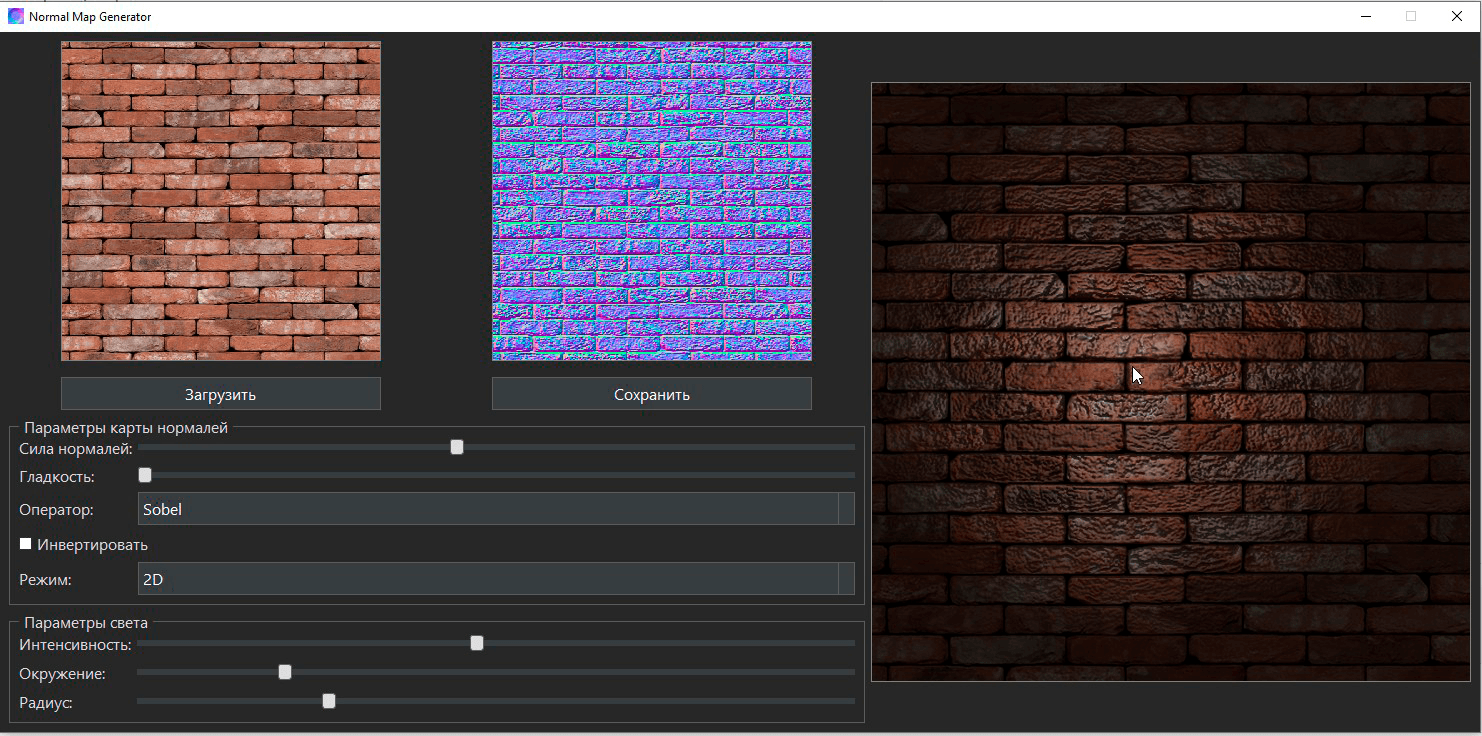
\includegraphics[width=1\linewidth]{testsave}}
	\caption{Загрузка изображения}
	\label{testsave:image}
\end{figure}

\subsubsection{Загрузка неподдерживаемого файла}

Сценарий: пользователь выбирает файл с неподдерживаемым расширением, например .txt или .mp3.

Ожидаемый результат: программа сообщает о невозможности загрузки изображения. Интерфейс остаётся стабильным.

Фактический результат: выведено сообщение об ошибке, работа программы не прерывается.

Результат системного тестирования представлен на рисунке \ref{testnoimage:image}.

\begin{figure}[H]
	\center{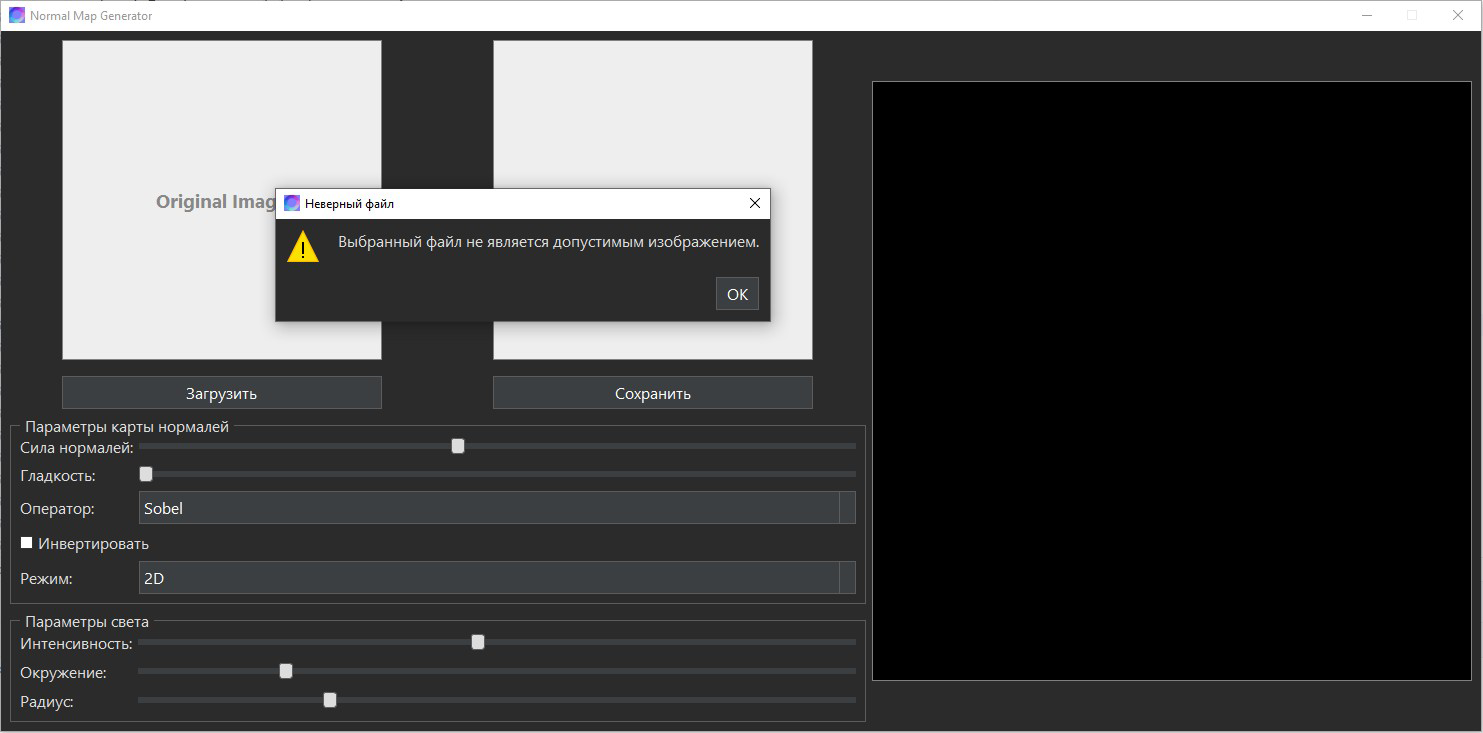
\includegraphics[width=1\linewidth]{testnoimage}}
	\caption{Загрузка неподдерживаемого файла}
	\label{testnoimage:image}
\end{figure}

\subsubsection{Изменение параметров генерации}

Сценарий: пользователь изменяет значение ползунка «Сила нормалей» и «Гладкость», переключает оператор градиента.

Ожидаемый результат: карта нормалей в окне визуализации обновляется в реальном времени при любом изменении параметров.

Фактический результат: визуализация обновляется мгновенно. Все изменения корректно отражаются на результатах.
\newpage
Результат системного тестирования представлен на рисунке \ref{testupstr:image}.

\begin{figure}[H]
	\center{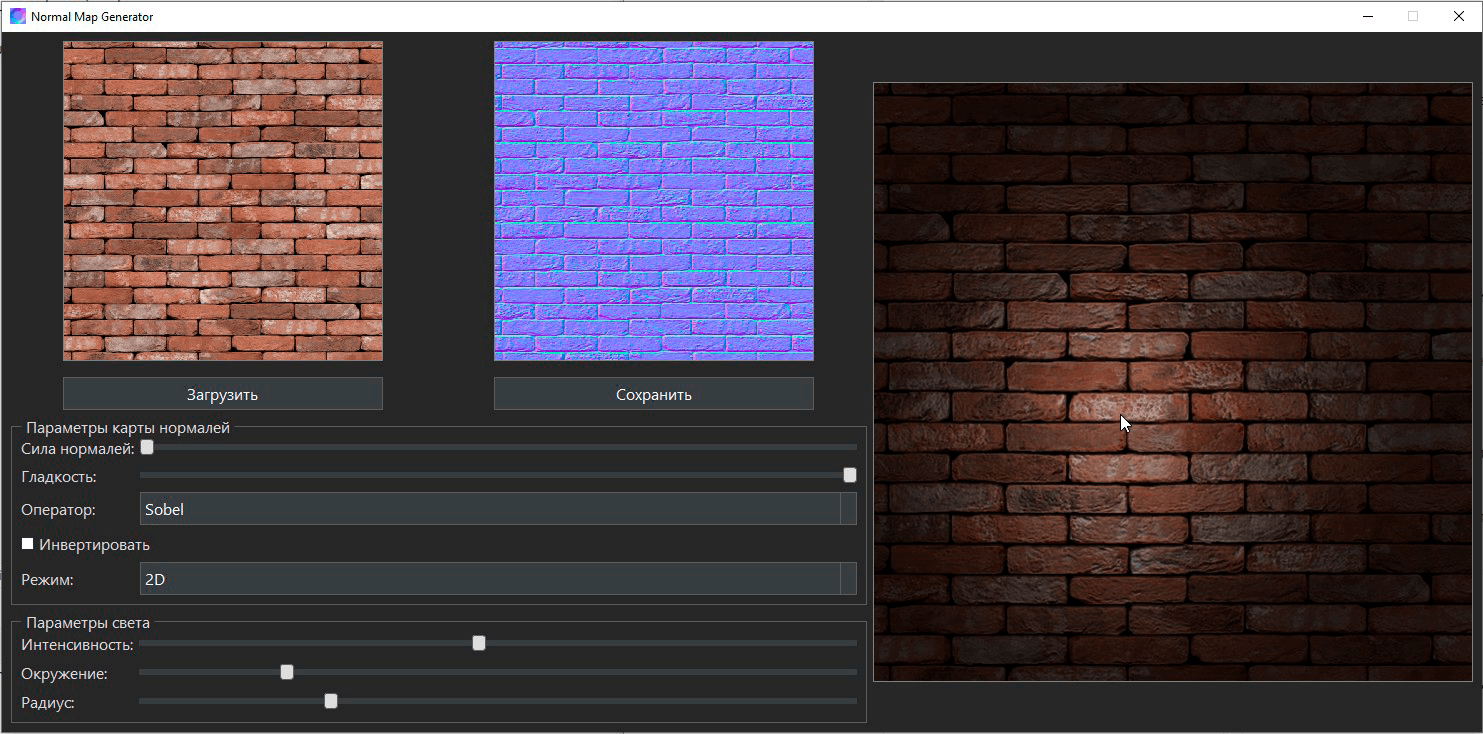
\includegraphics[width=1\linewidth]{testupstr}}
	\caption{Изменение параметров генерации}
	\label{testupstr:image}
\end{figure}

\subsubsection{Сохранение карты нормалей}

Сценарий: пользователь нажимает кнопку «Сохранить» и выбирает путь на диске.

Ожидаемый результат: файл с изображением карты нормалей сохраняется по указанному пути.

Фактический результат: изображение сохраняется корректно, без потери качества.
\newpage
Результат системного тестирования представлен на рисунке \ref{testsavenm:image}.

\begin{figure}[H]
	\center{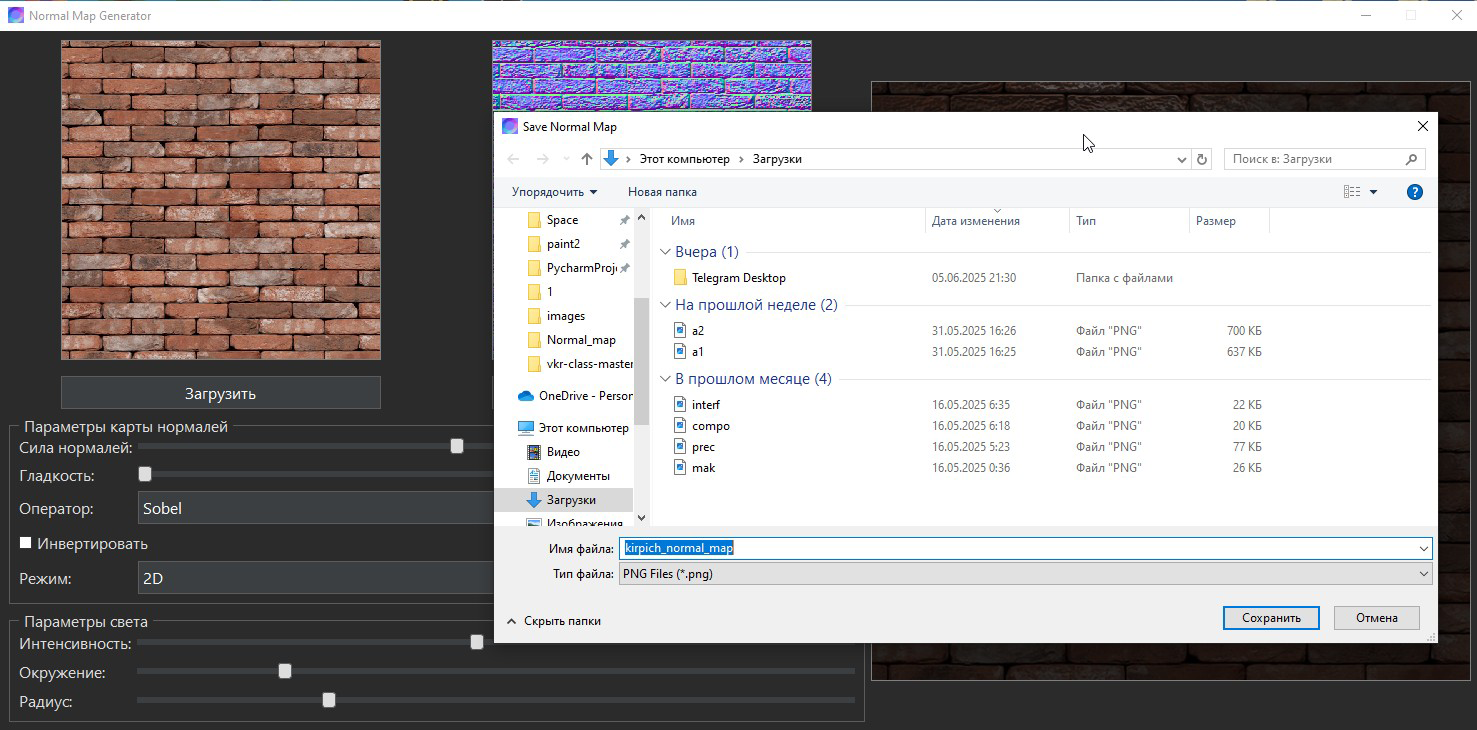
\includegraphics[width=1\linewidth]{testsavenm}}
	\caption{Сохранение карты нормалей}
	\label{testsavenm:image}
\end{figure}

\subsubsection{Изменение параметров света}

Сценарий: пользователь изменяет значение ползунка «Интенсивность», «Окружение» и «Радиус».

Ожидаемый результат: карта нормалей в окне визуализации обновляется в соответствии с новыми параметрами света.

Фактический результат: визуализация обновляется мгновенно. Все изменения корректно отражаются на результатах.
\newpage
Результат системного тестирования представлен на рисунке \ref{testint:image}.

\begin{figure}[H]
	\center{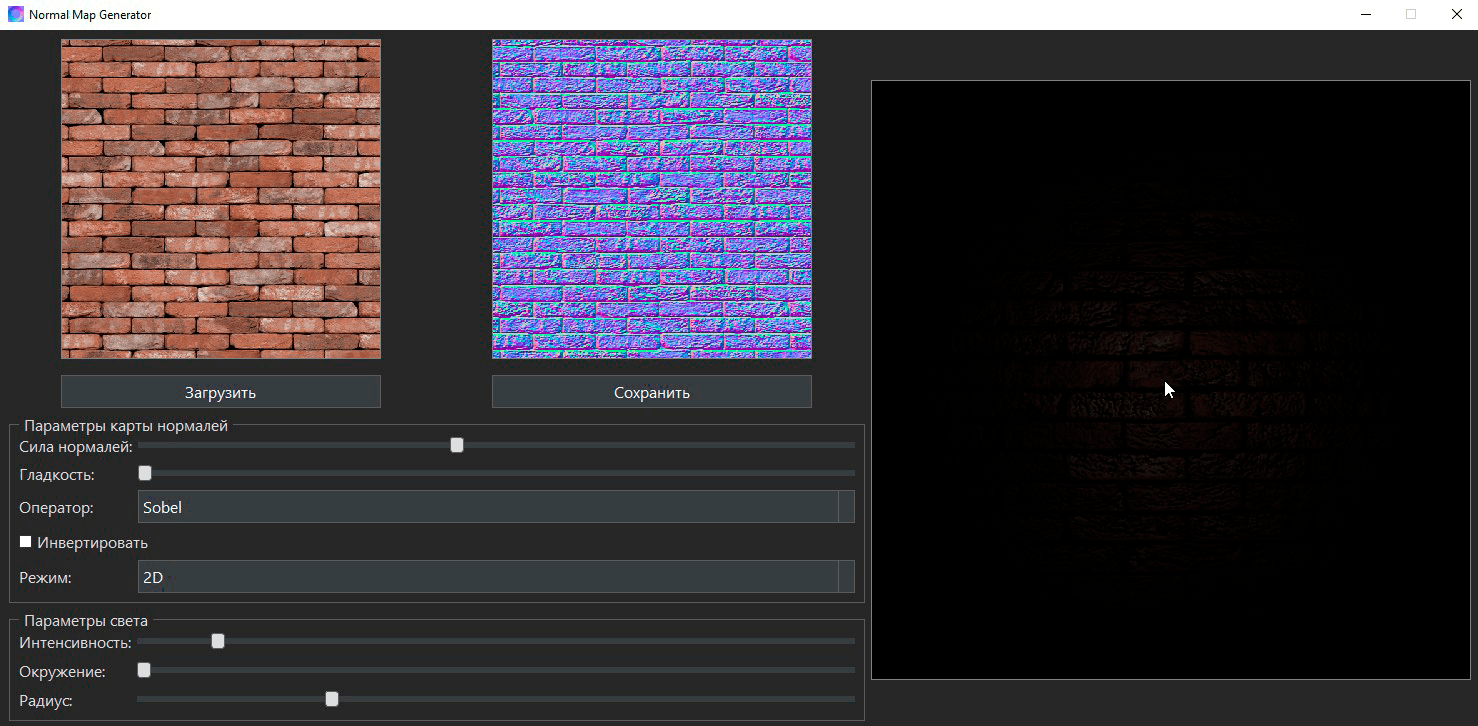
\includegraphics[width=1\linewidth]{testint}}
	\caption{Изменение параметров света}
	\label{testint:image}
\end{figure}

\subsubsection{Работа 3D-режима визуализации}

Сценарий: пользователь выбирает в выпадающем списке режим «3D». Отображается куб с наложенным изображением и освещением. Пользователь вращает куб, используя мышь.

Ожидаемый результат: куб вращается, направление света остаётся постоянным, тени на поверхностях меняются в зависимости от нормалей. Все грани текстурированы корректно.

Фактический результат: 3D-визуализация работает плавно. При перемещении мыши куб вращается без задержек. Световое пятно перемещается согласно направлению нормалей.
\newpage
Результат системного тестирования представлен на рисунке \ref{test3d:image}.

\begin{figure}[H]
	\center{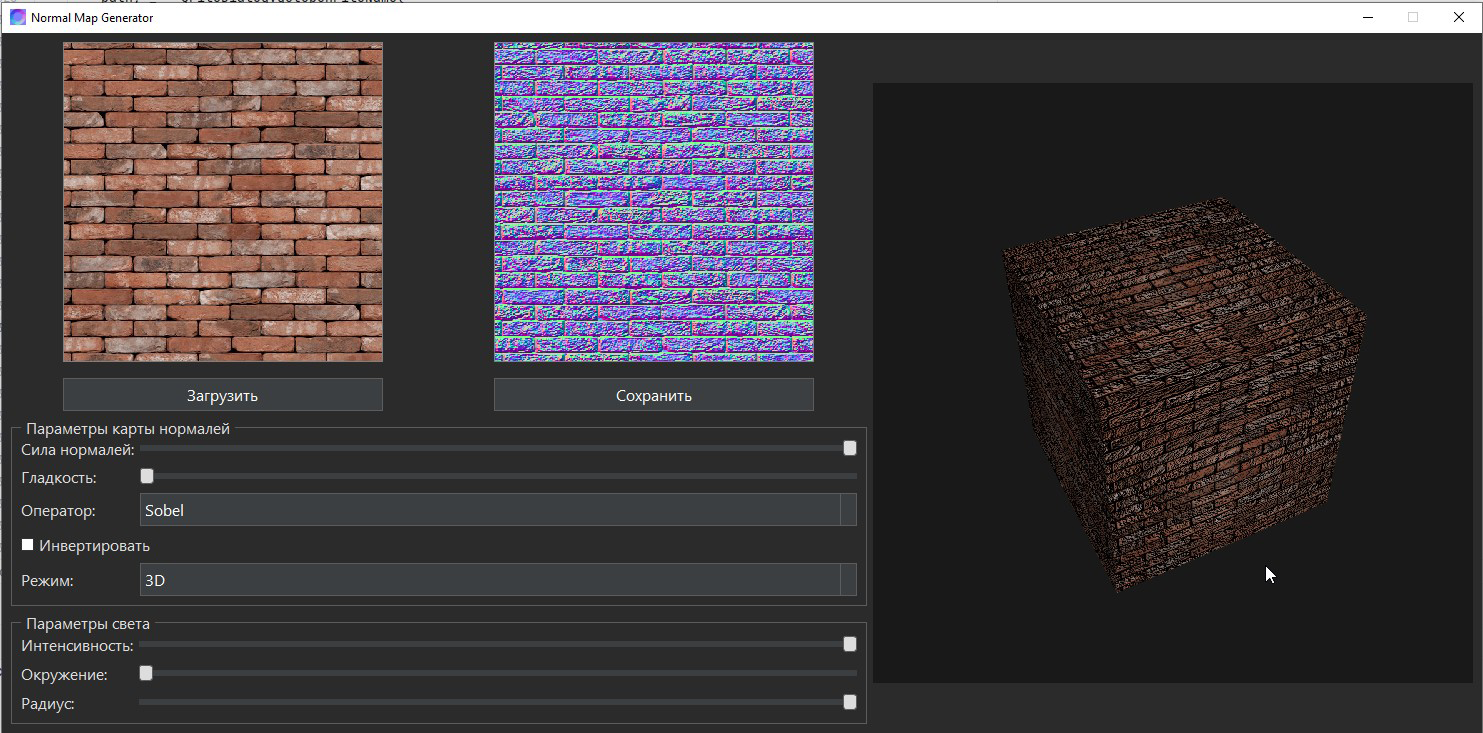
\includegraphics[width=1\linewidth]{test3d}}
	\caption{Работа 3D-режима визуализации}
	\label{test3d:image}
\end{figure}

\subsubsection{Быстрое переключение между 2D и 3D режимами}

Сценарий: пользователь быстро переключается между режимами отображения.

Ожидаемый результат: переключение проходит корректно, программа не зависает и не теряет данные.

Фактический результат: режимы переключаются без ошибок. Все параметры сохраняются при переходе между режимами.
\newpage
Результат системного тестирования представлен на рисунке \ref{testswap:image}.

\begin{figure}[H]
	\center{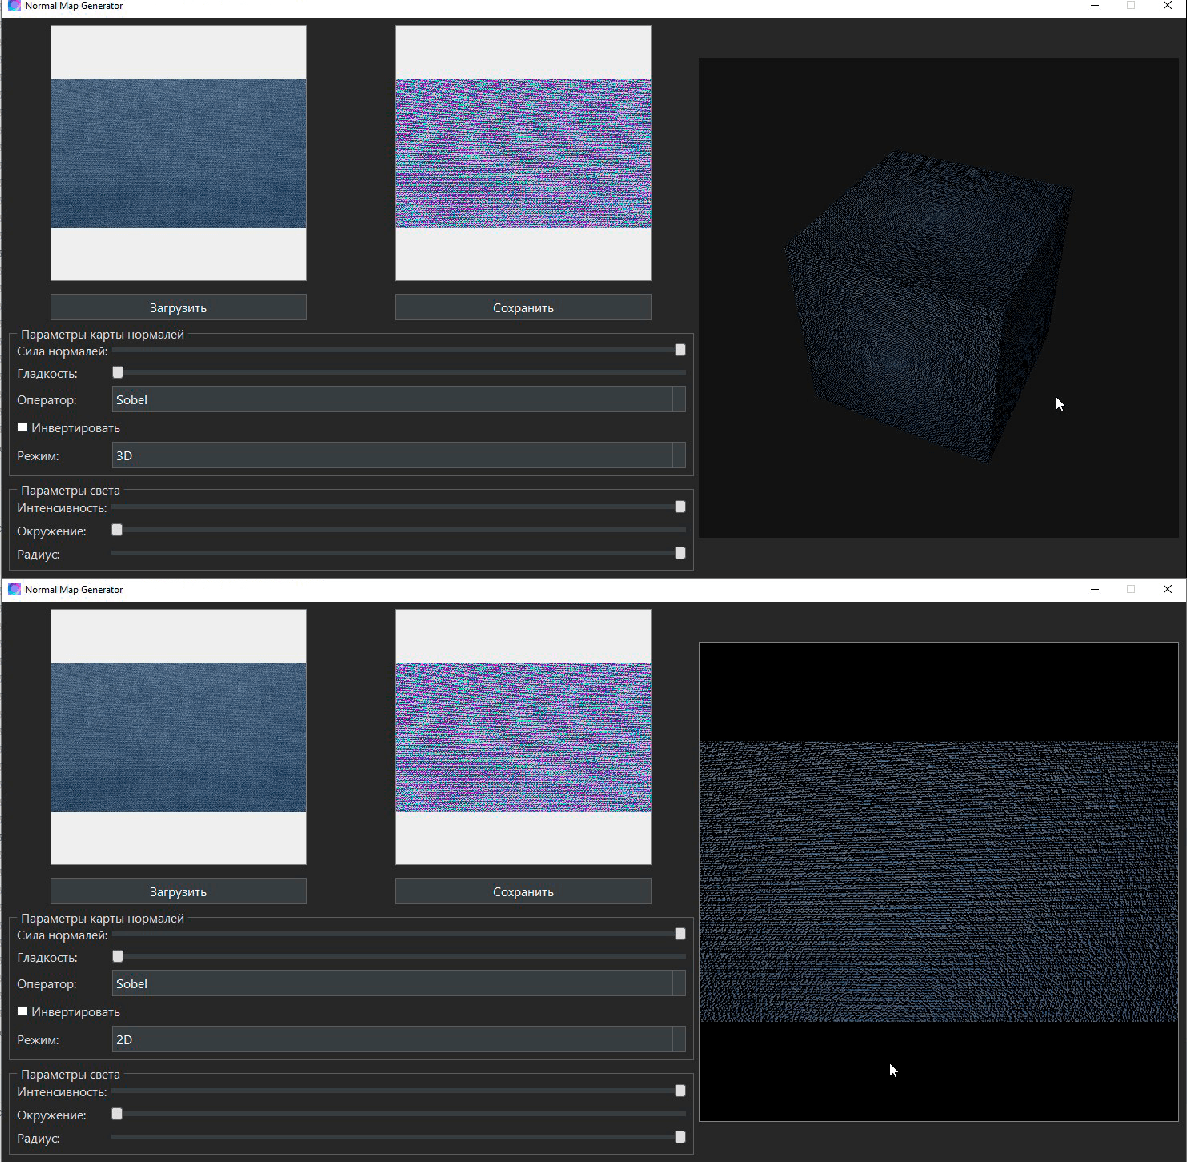
\includegraphics[width=1\linewidth]{testswap}}
	\caption{Быстрое переключение между 2D и 3D режимами}
	\label{testswap:image}
\end{figure}

\subsubsection{Обработка изображения с высоким разрешением}

Сценарий: пользователь загружает изображение высокого разрешения (например, 4096×4096 пикселей).

Ожидаемый результат: программа не принимает изображение, если его разрешение больше 2048×2048. Пользователь получает предупреждение.

Фактический результат: программа не обработала изображение. Появляется предупреждение с информацией о допустимых размерах.
\newpage
Результат системного тестирования представлен на рисунке \ref{testbig:image}.

\begin{figure}[H]
	\center{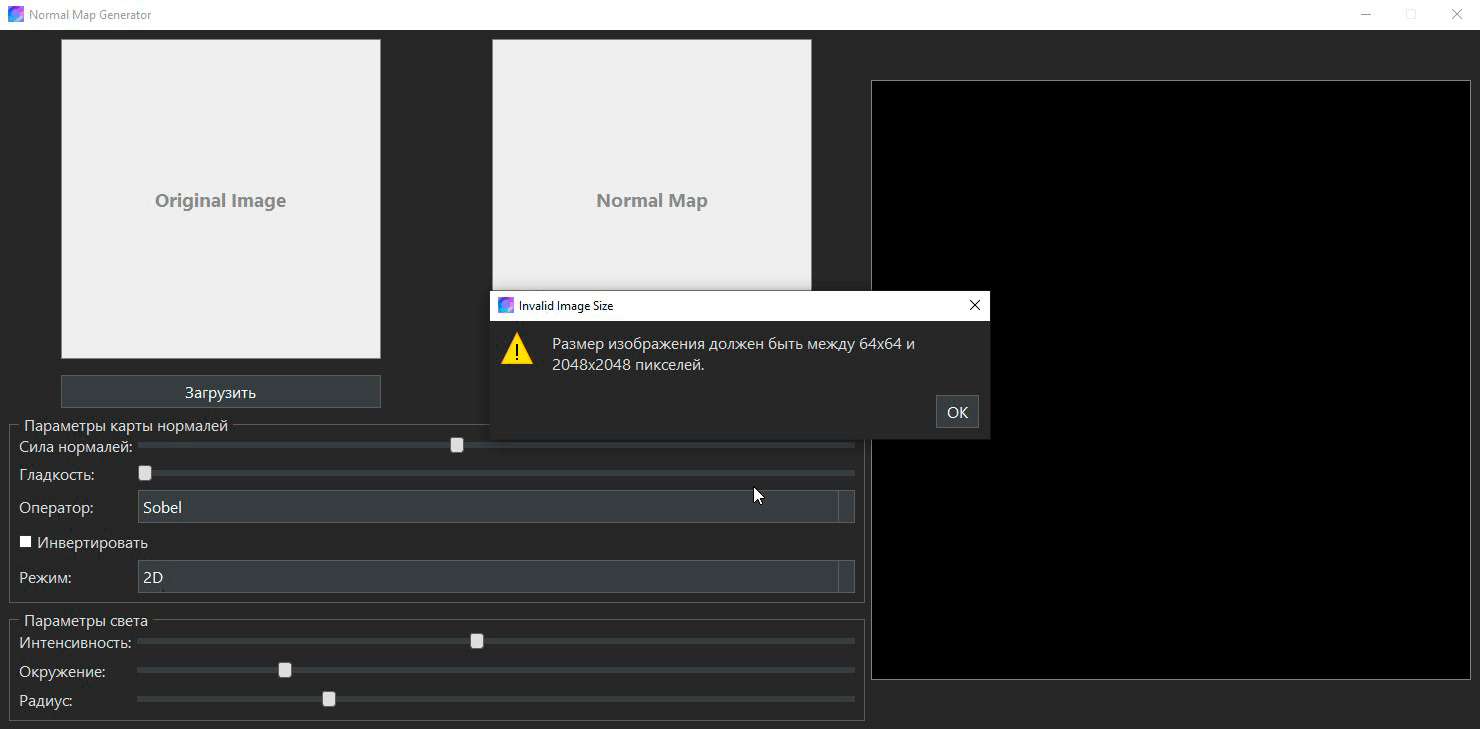
\includegraphics[width=1\linewidth]{testbig}}
	\caption{Обработка изображения с высоким разрешением}
	\label{testbig:image}
\end{figure}

\subsubsection{Инверсия карты нормалей}

Сценарий: пользователь активирует чекбокс «Инвертировать нормали».

Ожидаемый результат: отображение карты нормалей и визуализация освещения изменяются соответствующим образом — направления нормалей инвертируются.

Фактический результат: результат изменяется корректно, визуально ощущается изменение направления света на изображении.
\newpage
Результат системного тестирования представлен на рисунке \ref{testinv:image}.

\begin{figure}[H]
	\center{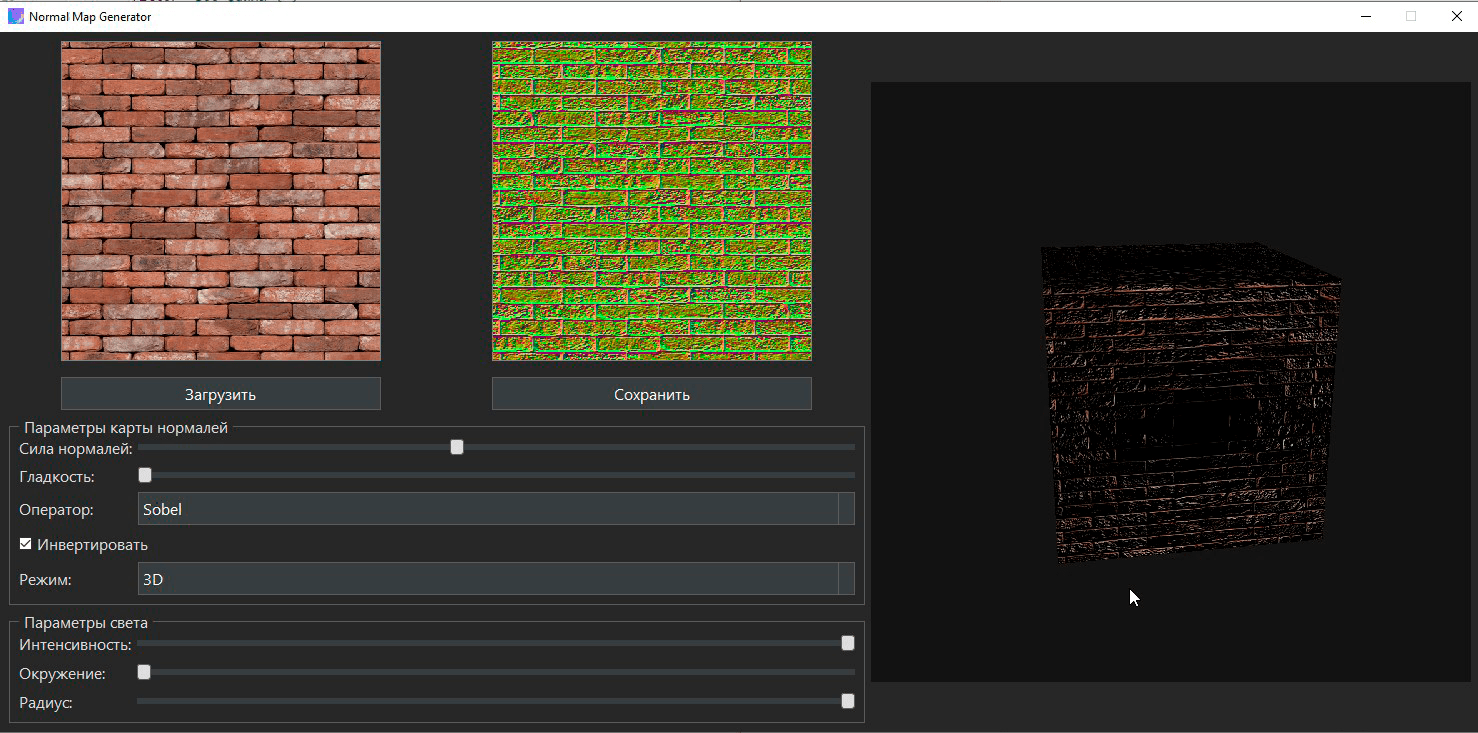
\includegraphics[width=1\linewidth]{testinv}}
	\caption{Инверсия карты нормалей}
	\label{testinv:image}
\end{figure}

\subsubsection{Перемещение источника света в режиме 2D}

Сценарий: пользователь перемещает курсор мыши по области визуализации в 2D-режиме.

Ожидаемый результат: освещение на изображении изменяется в соответствии с положением мыши — «фонарик» движется, создавая эффект направления света.

Фактический результат: реакция на перемещение мыши плавная, освещение обновляется в реальном времени.
\newpage
Результат системного тестирования представлен на рисунке \ref{testfon:image}.

\begin{figure}[H]
	\center{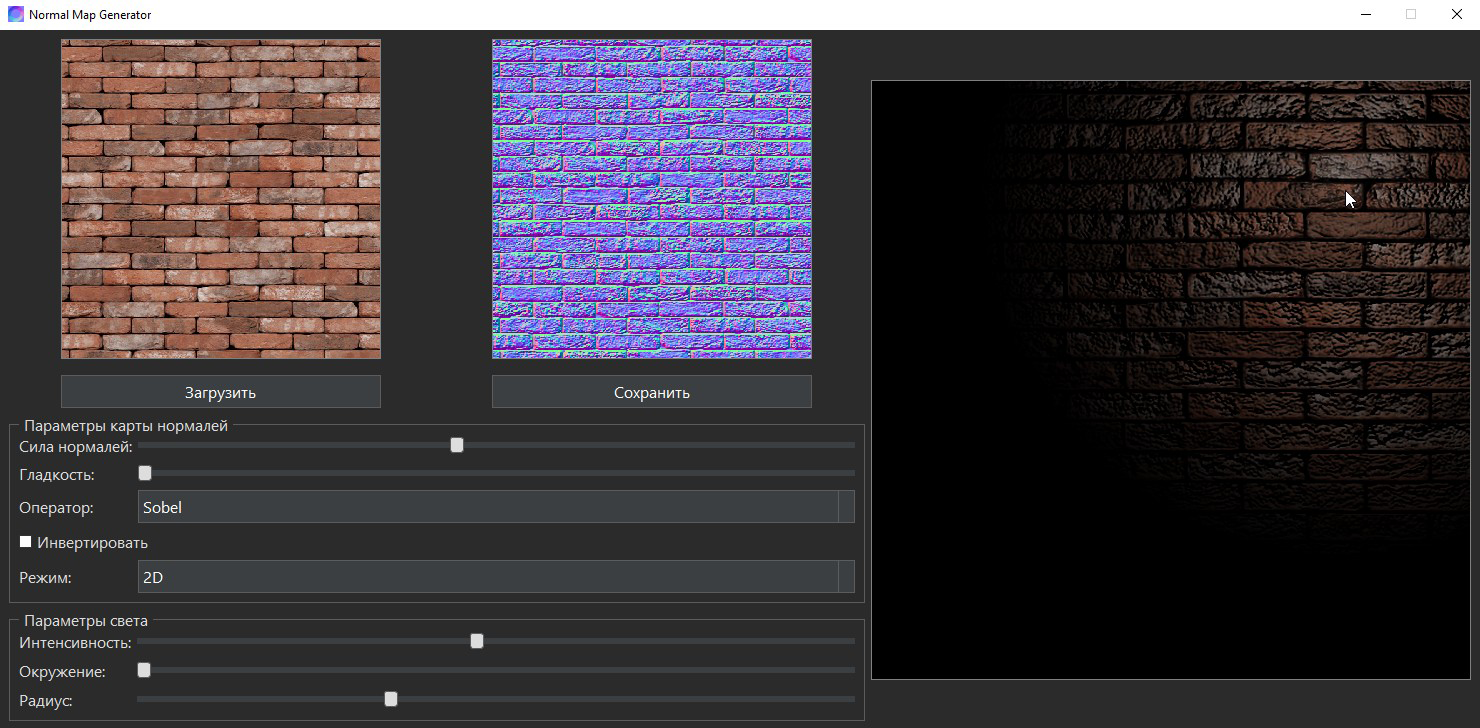
\includegraphics[width=1\linewidth]{testfon}}
	\caption{Перемещение источника света в режиме 2D}
	\label{testfon:image}
\end{figure}

\begin{comment}
На рисунке \ref{main:image} представлена главная страница сайта «Русатом – Аддитивные технологии».
\newpage % при необходимости можно переносить рисунок на новую страницу
\begin{figure}[H] % H - рисунок обязательно здесь, или переносится, оставляя пустоту
\center{\includegraphics[width=1\linewidth]{main1}}
\center{\includegraphics[width=1\linewidth]{main2}}
\center{\includegraphics[width=1\linewidth]{main3}}
\caption{Главная страница сайта «Русатом – Аддитивные технологии»}
\label{main:image}
\end{figure}

На рисунке \ref{menu:image} представлен динамический вывод заголовков, включающий в себя искомые фразы при поиске фраз.

\begin{figure}[ht]
\center{\includegraphics[width=1\linewidth]{menu}}
\caption{Динамический вывод заголовков}
\label{menu:image}
\end{figure}

На рисунке \ref{enter:image} представлен ввод данных для публикации новости.

\begin{figure}[ht]
\center{\includegraphics[width=1\linewidth]{enter}}
\caption{Ввод данных для публикации очень-очень длинной, интересной и полезной новости}
\label{enter:image}
\end{figure}
\end{comment}
   \section*{ЗАКЛЮЧЕНИЕ}
\addcontentsline{toc}{section}{ЗАКЛЮЧЕНИЕ}

Современные технологии обработки изображений и генерации нормалей находят всё более широкое применение в таких сферах, как компьютерная графика, визуализация, моделирование и разработка игр. В ходе выполнения данной выпускной квалификационной работы была спроектирована и реализована программная система, обеспечивающая построение карт нормалей из 2D-изображений и их интерактивную визуализацию.

Основные результаты работы:

\begin{enumerate}
	\item Выполнен анализ предметной области, охватывающей задачи генерации карт нормалей и их применения в визуальных приложениях.
	\item Разработана концептуальная модель программного решения, определены функциональные и нефункциональные требования к системе.
	\item Спроектирован и реализован пользовательский интерфейс, обеспечивающий интуитивную работу с изображениями, настройку параметров генерации и визуализации.
	\item Внедрены режимы двухмерной и трёхмерной визуализации с возможностью симуляции освещения на основе нормалей.
	\item Проведено тестирование программной системы, подтверждающее её работоспособность и соответствие заданным требованиям.
\end{enumerate}

Поставленные задачи были успешно решены. Результатом работы стала программа с графическим интерфейсом, позволяющая пользователю не только генерировать карты нормалей из изображений, но и анализировать их в интерактивном режиме с управляемыми параметрами освещения.

Полученные результаты демонстрируют практическую ценность выполненной разработки и подтверждают успешное достижение поставленных в начале проекта целей.


}\fi
\addcontentsline{toc}{section}{СПИСОК ИСПОЛЬЗОВАННЫХ ИСТОЧНИКОВ}

\begin{thebibliography}{9}

    \bibitem{gambetta2021}
    Гамбетта, Г. Компьютерная графика с нуля / Г. Гамбетта. – Сан-Франциско: No Starch Press, 2021. – 248 с. – ISBN 978-1-7185-0076-1. – Текст: непосредственный.
    
    \bibitem{lukacs2020}
    Лукач, Р.; Платаниотис, К. Н. (ред.) Обработка цветных изображений: методы и приложения / под ред. Р. Лукача, К. Н. Платаниотиса. – Бока-Ратон: CRC Press, 2020. – 560 с. – ISBN 978-0-8493-7491-4. – Текст: непосредственный.
    
    \bibitem{reed2020}
    Рид, Т. Р. (ред.) Цифровая последовательность изображений: методы и приложения / под ред. Т. Р. Рида. – Нью-Йорк: Springer, 2020. – 400 с. – ISBN 978-0-387-94854-6. – Текст: непосредственный.
    
    \bibitem{thalmann2021}
    Магненат-Тальманн, Н. (ред.) Достижения в компьютерной графике: материалы 38-й Международной конференции по компьютерной графике CGI 2021 / под ред. Н. Магненат-Тальманн. – Чам: Springer, 2021. – 392 с. – ISBN 978-3-030-89028-5. – Текст: непосредственный.
    
    \bibitem{martins2024}
    Мартинс, К. Обработка изображений и компьютерное зрение / К. Мартинс. – Амазон: Amazon KDP, 2024. – 150 с. – ISBN 978-1-23456-789-0. – Текст: непосредственный.
    
    \bibitem{distante2020}
    Дистанте, А.; Дистанте, К. Учебное пособие по обработке изображений и компьютерному зрению: том 1 – от энергии к изображению / А. Дистанте, К. Дистанте. – Чам : Springer, 2020. – 491 с. – ISBN 978‑3‑030‑38147‑9. – Текст: непосредственный.
    
    \bibitem{ansari2024}
    Ансари, И. А.; Баджадж, В. Обработка изображений с использованием Python: практический подход / И. А. Ансари, В. Баджадж. – Лондон: IOP Publishing, 2024. – 350 с. – ISBN 978-0-7503-5924-5. – Текст: непосредственный.
    
    \bibitem{bruno2024}
    Бруно, А.; Маццео, П. Л.; Куэвас, Ф. Цифровая обработка изображений: последние достижения и приложения / А. Бруно, П. Л. Маццео, Ф. Куэвас. – Лондон: IOP Publishing, 2024. – 234 с. – ISBN 978-0-85466-491-7. – Текст: непосредственный.
    
    \bibitem{umbaugh2022}
    Умбау, С. Э. Цифровая обработка и анализ изображений: улучшение, восстановление и сжатие цифровых изображений / С. Э. Умбау. – Эдвардсвилл: CRC Press, 2022. – 928 с. – ISBN 978-1-032-07130-5. – Текст: непосредственный.
    
    \bibitem{tyagi2021}
    Тьяги, В. Понимание цифровой обработки изображений / В. Тьяги. – Лондон: Taylor \& Francis, 2021. – 368 с. – ISBN 978-0-367-78082-1. – Текст: непосредственный.
    
    \bibitem{matveev2023}
    Матвеев, А. И. Цифровая обработка изображений в OpenCV. Практикум: учебное пособие. – 2-е изд., стереотип. – СПб.: Лань, 2023. – 104 с. – ISBN 978-5-507-46249-0. – Текст: непосредственный.
    
    \bibitem{baskar2023}
    Баскар, А.; Раджаппа, М.; Васудеван, Ш. К.; Муругеш, Т. С. Цифровая обработка изображений / А. Баскар, М. Раджаппа, Ш. К. Васудеван, Т. С. Муругеш. – Лондон: Chapman \& Hall, 2023. – 208 с. – ISBN 978-1-032-10857-5. – Текст: непосредственный.
    
    \bibitem{yane2021}
    Яне, Б. Цифровая обработка изображений: Концепции, алгоритмы и научные приложения / Б. Яне. – Берлин: Springer, 2021. – 600 с. – ISBN 978-3-662-21818-1. – Текст: непосредственный.
    
    \bibitem{shafik2020}
    Шафик, С.; Машкур, А.; Майр-Дорн, К.; Эгед, А. Машинное обучение в разработке программного обеспечения: систематический обзор / С. Шафик и др. – arXiv, 2020. – 30 с. – arXiv:2005.13299. – Текст: непосредственный.
    
    \bibitem{jehangiri2024}
    Жехангири, З. М.; Шахзад, М.; Хан, У. (ред.) Цифровая обработка изображений: передовые технологии и приложения / под ред. З. М. Жехангири, М. Шахзад, У. Хан. – Базель: MDPI, 2024. – 348 с. – ISBN 978-3-7258-1825-9. – Текст: непосредственный.
    
    \bibitem{farinella2020}
	Фаринелла, Дж. М. и др. (ред.) Компьютерное зрение, визуализация и теория компьютерной графики: материалы 15-й Международной конференции VISIGRAPP 2020 / под ред. Дж. М. Фаринелла и др. – Чам: Springer, 2020. – 392 с. – ISBN 978-3-030-94893-1. – Текст: непосредственный.
    
    \bibitem{matiz2020}
    Мэтиз, Э. Изучаем Python: программирование игр, визуализация данных, веб-приложения / Э. Мэтиз. – СПб.: Питер, 2020. – 512 с. – ISBN 978-5-4461-0923-4. – Текст: непосредственный.
    
    \bibitem{johnson2020}
    Джонсон, Д. Проектирование с учетом пользователя: простое руководство по пониманию принципов проектирования пользовательского интерфейса / Д. Джонсон. – Амстердам: Morgan Kaufmann, 2020. – 250 с. – ISBN 978-0-12-818202-4. – Текст: непосредственный.
    
    \bibitem{ramalho2022}
    Рамальо, Л. Глубокое освоение Python (2-е издание) / Л. Рамальо. – Себастопол: O’Reilly Media, 2022. – 1012 с. – ISBN 978-1-4920-4604-0. – Текст: непосредственный.
    
    \bibitem{dawson2021}
    Доусон, М. Программируем на Python / М. Доусон. – М.: Вильямс, 2021. – 400 с. – ISBN 978-5-8459-7890-1. – Текст: непосредственный.
    
    \bibitem{tidwell2020}
    Тидвелл, Дж.; Брюэр, К.; Валенсия, А. Проектирование интерфейсов (3-е издание) / Дж. Тидвелл, К. Брюэр, А. Валенсия. – Себастопол: O’Reilly Media, 2020. – 560 с. – ISBN 978-1-4920-6832-5. – Текст: непосредственный.
    
    \bibitem{prokhorenok2021}
    Прохоренок, Н. А.; Дронов, В. А. Python 3 и PyQt 5. Разработка приложений. – 2-е изд., перераб. и доп. – СПб.: БХВ-Петербург, 2021. – 832 с. – ISBN 978-5-9775-3978-4. – Текст: непосредственный.
    
    \bibitem{cooper2020}
    Купер, А.; Райман, Р.; Кронин, Д. Внимание к интерфейсу: основы проектирования взаимодействия (4-е издание) / А. Купер, Р. Райман, Д. Кронин. – Индианаполис: Wiley, 2020. – 720 с. – ISBN 978-1-118-76457-3. – Текст: непосредственный.
    
    \bibitem{ravichandiran2020}
    Равичандиран, С. Глубокое обучение с подкреплением на Python / С. Равичандиран. – Москва: ДМК Пресс, 2020. – 450 с. – ISBN 978-5-97060-789-2. – Текст: непосредственный.
    
    \bibitem{talipov2020}
    Талипов, С. Н. Программирование на Python3 с PyQt5. – Екатеринбург: Уральское издательство, 2020. – 155 с. – ISBN 978-5-04-350119-6. – Текст: непосредственный.
    
    \bibitem{kaehler2021}
    Кэлер, А.; Брэдски, Г. Изучаем OpenCV 4 / А. Кэлер, Г. Брэдски. – Лондон: DМК Пресс, 2021. – 850 с. – ISBN 978‑5‑97060‑999‑9. – Текст: непосредственный.
    
    \bibitem{russ2020}
    Русс, Дж. К.; Нил, Ф. Б. Справочник по обработке изображений / Дж. К. Русс, Ф. Б. Нил. – Лондон: CRC Press, 2020. – 1032 с. – ISBN 978-1-4822-3959-0. – Текст: непосредственный.
    
    \bibitem{day2021}
    Дей, С. Мастер-класс по обработке изображений с использованием Python: 50+ решений и техник / С. Дей. – Нью-Дели: BPB Publications, 2021. – 450 с. – ISBN 978-93-89898-64-1. – Текст: непосредственный.
    
    \bibitem{ahmed2021}
    Ахмед, З.; Алмусаллам, С.; Уилсон, К. Автоматизация модульного тестирования на Python / З. Ахмед, С. Алмусаллам, К. Уилсон. – Нью‑Йорк: Springer, 2021. – 300 с. – ISBN 978‑1‑4842‑7854‑3. – Текст: непосредственный.
    
    \bibitem{sharma2023}
    Шарма, М. Стратегии тестирования ПО для 2020‑х / М. Шарма. – Бирмингем: Packt Publishing, 2023. – 265 с. – ISBN 978‑1‑83763‑802‑4. – Текст: непосредственный.
    
    
\end{thebibliography}

\ifВКР{\appendix{Представление графического материала}

Графический материал, выполненный на отдельных листах,
изображен на рисунках А.1--А.\arabic{числоПлакатов}.
\setcounter{числоПлакатов}{0}

\renewcommand{\thefigure}{А.\arabic{figure}} % шаблон номера для плакатов

\begin{landscape}

\begin{плакат}
    \includegraphics[width=0.82\linewidth]{Ramka1.png}
    \заголовок{Сведения о ВКРБ}
    \label{pl1:image}      
\end{плакат}

\begin{плакат}
    \includegraphics[width=0.82\linewidth]{Ramka2.png}
    \заголовок{Цель и задачи разработки}
    \label{pl2:image}      
\end{плакат}

\begin{плакат}
    \includegraphics[width=0.82\linewidth]{Ramka3.png}
    \заголовок{Диаграмма прецендентов}
    \label{pl3:image}      
\end{плакат}

\begin{плакат}
    \includegraphics[width=0.82\linewidth]{Ramka4.png}
    \заголовок{Диаграмма компонентов}
    \label{pl4:image}      
\end{плакат}

\begin{плакат}
	\includegraphics[width=0.82\linewidth]{Ramka5.png}
	\заголовок{Диаграмма классов}
	\label{pl5:image}      
\end{плакат}

\begin{плакат}
	\includegraphics[width=0.82\linewidth]{Ramka6.png}
	\заголовок{Макет приложения}
	\label{pl6:image}      
\end{плакат}

\begin{плакат}
	\includegraphics[width=0.82\linewidth]{Ramka7.png}
	\заголовок{Интерфейс приложения}
	\label{pl7:image}      
\end{плакат}

\begin{плакат}
	\includegraphics[width=0.82\linewidth]{Ramka8.png}
	\заголовок{Заключение}
	\label{pl8:image}      
\end{плакат}

\end{landscape}
}\fi
\ifПрактика{}\else{\appendix{Фрагменты исходного кода программы}

main.tex
\lstinputlisting[language=Tex, frame=none]{main.tex}

ТехПроект.tex
\lstinputlisting[language=Tex, frame=none]{ТехПроект.tex}

\ifВКР{
\newpage
\addcontentsline{toc}{section}{На отдельных листах (CD-RW в прикрепленном конверте)}
\noindent
\begin{tabular}{p{5.8cm}C{4.8cm}C{4.8cm}}
   Автор ВКР & \lhrulefill{\fill} & \fillcenter\Автор \\
            \setarstrut{\footnotesize}
           & \footnotesize{(подпись, дата)} & \\
            \restorearstrut
   Руководитель ВКР & \lhrulefill{\fill} & \fillcenter\Руководитель \\
            \setarstrut{\footnotesize}
           & \footnotesize{(подпись, дата)} & \\
            \restorearstrut
   Нормоконтроль & \lhrulefill{\fill} & \fillcenter\Нормоконтроль \\
            \setarstrut{\footnotesize}
           & \footnotesize{(подпись, дата)} & \\
            \restorearstrut
\end{tabular}
\vskip 2cm
\begin{center}
\textbf{Место для диска}
\end{center}
}\fi
}\fi
\end{document}
